\chapter{复数系}

在数学中,数是最基础、应用最广泛的工具之一,我们已经在自然数的基础上,逐步学习了整数、有理数、实数等概念和它们的运算及性质.这一章,我们将进一步学习复数的概念及其运算、性质.

\section{复数的概念}
\subsection{数的概念的发展}

数的概念是中学数学的主要内容之一,是从实践中逐步形成和发展起来的.早在有文字记载的历史以前,由于计数和排序的需要,人类就建立起自然数(正整数)的概念,处理着各种常见的、有天然单元的可数量. 自然数的全体构成了自然数集$\mathbb{N}$.

随着社会生产和科学技术的发展,数的概念相应地得到了不断发展.

为了处理实践中遇到的测量、分割、分配等可以细分的量,人们引进了正分数;为了解决生产实践中的各种具有相反意义的量的表示和运算问题,人们又引进了零及负数,并把自然数看作正整数. 这样一来,把正整数、零、负整数合并在一起,称为整数集$\mathbb{Z}$;并把整数与分数(正分数、负分数)合称为有理数集$\mathbb{Q}$.

任一有理数,可以表示成分数形式$\frac{m}{n}$,其中$m,n\in\mathbb{N}$; 还可以表示成循环小数(包括循环节为0的小数).

有理数系的形成,使得许多人曾认为这就足以解决可度量的量,特别是在古希腊,他们曾认为:任意两条线段都是可公度的(即:任意两条线段长度的比都是有理数). 但实际上这种认识是不正确的. 例如,正方形的边长和对角线长,正五边形的边长和对角线长都是不可公度的. 为了解决这些量与量之比值不能用有理数表示的矛盾,于是又引进了无理数的概念,无理数就是无限不循环小数. 无理数与有理数统称为实数,构成了实数集$\mathbb{R}$.

实数集$\mathbb{R}$对加、减、乘、除(零不作除数)四则运算是封闭的,且满足运算通性,即满足加、乘法的交换律、结合律和分配律,数零与1保持在运算中的特性.

实数集$\mathbb{R}$与数轴上的点集之间,可以建立起一一对应的关系. 因此,从度量的角度来说,实数系是一个完整无缺的数系,它足以满足度量的实际需要.

但是,从代数运算和解方程的角度来看,实数集并不完整无缺,因为,在实数范围内,开方运算并不封闭,实系数方程(如$ax^2+bx+c=0$)在实数系内未必有解.

事实上,数的概念的逐步扩充,与代数运算和解方程的需要也是相适应的,例如:

由于自然数集$\mathbb{N}$对于减法、除法运算不封闭,因而方程$x+7=2$, $7x=5$等在自然数集中无解,但在有理数集$\mathbb{Q}$中就有解$x=-5$, $x=\frac{5}{7}$. 

由于有理数集$\mathbb{Q}$对于开方运算不封闭,因而方程$x^2-3
=0$在$\mathbb{Q}$中无解,但在实数集$\mathbb{R}$中就有两个解$x=\pm\sqrt{3}$.

同样,实数集$\mathbb{R}$对开方运算仍不封闭,因而象方程$x^2+1=0$在$\mathbb{R}$中还是无解,因为,没有一个实数的平方等于$-1$.要解决这一类矛盾,数的概念需要进一步发展,这就需要引进新数,并讨论它的运算.

\begin{ex}
\begin{enumerate}
    \item 试叙述实数集$\mathbb{R}$中有哪些数系运算通性?
\item 试分别在自然数集$\mathbb{N}$.整数集$\mathbb{Z}$、有理数集$\mathbb{Q}$和实数集$\mathbb{R}$中,解方程$(x-2)(3x+1)(x+7)(x^2+5)=0$.
\end{enumerate}
\end{ex}

\subsection{复数及其几何表示}
如上所述,由于解方程的需要,早在十六世纪,人们就引进了一个新数$i$,使得方程有解,并把它叫做\textbf{虚数单位},并规定:
\begin{enumerate}[(1)]
\item $i^2=-1$;
\item 它与实数进行四则运算时,运算通性及数0与1的运算特性仍然保持. 即,满足加、乘法的交换律、结合律、分配律;满足
\[\begin{split}
    0+i&=i+0=i,\\
0\cdot i&=i\cdot 0=0,\\
1\cdot i&=i\cdot 1=i.
\end{split}\]
\end{enumerate}

在这样的规定下,$i$可以与实数$b$相乘,再与实数$a$相加,从而得到$a+bi$.

这样,数的概念扩大了,我们就把形如$a+bi\; (a,b\in\mathbb{R})$的数,叫做复数.全体复数构成的集合,称为\textbf{复数集},
一般记作$\mathbb{C}$.

对于复数$a+bi\; (a,b\in\mathbb{R})$,当$b=0$时,就是实数$a$;当$b\ne 0$时,这一复数叫做虚数,特别地,当$a=0$且$b\ne 0$时,叫做纯虚数.

$a$,$b$分别叫做复数$z=a+bi$的\textbf{实部}与\textbf{虚部},并且记作:${\rm Re}(z)=a$, ${\rm Im}(z)=b$.

显然,实数集$\mathbb{R}$是复数集$\mathbb{C}$的真子集,即$\mathbb{R}\subset \mathbb{C}$.

例如,$3+2i$, $-\frac{1}{2}-\sqrt{3}i$, $-0.25i$都是虚数. 其中$-0.25i$是纯虚数.它们的实部和虚部分别为:
\[\begin{split}
&{\rm Re}(3+2i)=3,\qquad {\rm Im}(3+2i)=2;\\
&{\rm Re}\left(-\frac{1}{2}-\sqrt{3}i\right)=-\frac{1}{2},\qquad {\rm Im}\left(-\frac{1}{2}-\sqrt{3}i\right)=-\sqrt{3};\\
&{\rm Re}(-0.25i)=0,\qquad {\rm Im}(-0.25i)=-0.25.\\
\end{split}\]

我们还规定,当且仅当两个复数的实部和虚部分别相等时,这两个复数相等,即
\[a+bi=c+di\Longleftrightarrow a=c\text{且}b=d\]
或
\[z_1=z_2\Longleftrightarrow {\rm Re}(z_1)={\rm Re}(z_2)\quad \text{且} \quad {\rm Im}(z_1)={\rm Im}(z_2)\]
特别地,我们可以得出
\[a+bi=0\Longleftrightarrow a=b=0\]

\begin{example}
    若$3x+2yi-1=(x-1)i+y$,其中$x,y\in\mathbb{R}$. 求$x$与$y$的值.
\end{example}

\begin{solution}
将已知等式整理得
\[(3x-1)+2yi=y+(x-1)i\]
根据复数相等的定义,可得方程组$\begin{cases}
    3x-1=y\\
    2y=x-1
\end{cases}$,
解得
\[x=\frac{1}{5},\qquad y=-\frac{2}{5}\]
\end{solution}

当两个复数的实部相等、虚部互为相反数时,这两个复数叫做\textbf{互为共轭复数},即
:复数$a+bi$与$a-bi$叫做互为共轭复数. 一般地,复数$z=a+bi$的共轭复数表示为:
$$\overline{z}=a-bi$$

显然,实数$a$(即虚部为零的复数)的共轭复数仍是它自身$a$.

我们已经知道,实数集与数轴上的点之间可建立一一对应关系. 引进虚数,构成复数集之后,是否有相应的对应关系呢?

首先,虚数单位$i$在实数轴上没有立足之地,它不属于实数集;其次,当$b\ne 0$时,复数$a+bi$也不可能在实数轴上找出对应之点,它仍不属于实数集,因此,我们必须另找途径来建立对应关系.

从复数及其相等的定义中,我们知道,任何一个复数
$z=a+bi$,都由一个有序实数对$(a,b)$唯一确定,而每一个有序实数对,又借助平面的坐标化可以唯一确定平面上一个点,因此,只要在平面上建立起直角坐标系,就可以用平面上的点$Z(a,b)$表示出复数$z=a+bi$,如图1.1所示.

\begin{minipage}{.45\textwidth}
\centering
\begin{tikzpicture}[>=stealth]
\draw[->](-1,0)--(3,0)node[right]{$x$};
\draw[->](0,-1)--(0,3)node[right]{$y$};
\draw[dashed](0,1.5)node[left]{$b$}--(2,1.5)node[above]{$Z(a,b)$}--(2,0)node[below]{$a$};
\node[below right]{$O$};
\draw[fill](2,1.5)circle(1pt);
\end{tikzpicture}
\captionof{figure}{ }
\end{minipage}
\hfill
\begin{minipage}{.45\textwidth}
\centering
    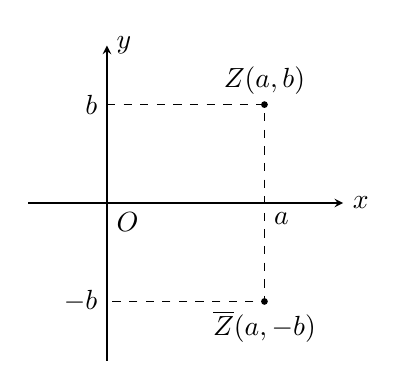
\begin{tikzpicture}[>=stealth]
  \draw[->](-1,0)--(3,0)node[right]{$x$};
\draw[->](0,-2)--(0,2)node[right]{$y$};
\draw[dashed](0,1.25)node[left]{$b$}--(2,1.25)node[above]{$Z(a,b)$}--(2,0)node[below right]{$a$}--(2,-1.25)node[below]{$\overline{Z}(a,-b)$}--(0,-1.25)node[left]{$-b$};
\node[below right]{$O$};  
\draw[fill](2,1.25)circle(1pt);
\draw[fill](2,-1.25)circle(1pt);
    \end{tikzpicture}
\captionof{figure}{ }
\end{minipage}


这个建立了坐标系来表示复数的平面,叫做\textbf{复平面},其中$X$轴叫做\textbf{实轴},$Y$轴(不含原点)叫做\textbf{虚轴}.

这样一来,每一个复数,在复平面内都有唯一一点和它对应,反之,复平面内的每一个点,都有唯一的一个复数和它对应,因此,复数集$\mathbb{C}$和复平面上的点集是一一对应的. 特别地,实数集和复平面实轴上的点集一一对应;纯虚数集合和复平面虚轴(不含原点)上的点集一一对应.

显然,互为共轭的两个复数$z=a+bi$与$\bar z=a-bi$在复平面上对应的两点$Z(a,b)$与$\overline{Z}(a,-b)$关于实轴对称(图1.2).

\begin{ex}
\begin{enumerate}
    \item 将下列给出的各数,分类填入表中:
\[1-\sqrt{2},\quad 0.618,\quad -1+i,\quad 0,\quad i,\quad i^2,\quad 3+7\sqrt{2}i\]
\[i-1,\quad (\sqrt{2}+\sqrt{3})i,\quad \sqrt{2}i-\sqrt{2},\quad -\frac{\sqrt{3}}{2}i\]
\begin{tabular}{|c|p{.7\textwidth}|}
\hline
    实数&\\
\hline
虚数&\\\hline
纯虚数&\\    \hline
\end{tabular}

\item 填写下列表格:
\begin{center}
\begin{tabular}{|c|p{.1\textwidth}|p{.1\textwidth}|p{.1\textwidth}|p{.1\textwidth}|p{.1\textwidth}|}
\hline 
复数$z$& ${\rm Re}(z)$& ${\rm Im}(z)$&$\bar z$& ${\rm Re}(\bar z)$& ${\rm Im}(\bar z)$\\
\hline
$-\sqrt{3}+i$ &&&&&\\
$-(1+\sqrt{2})$&&&&&\\
$\frac{i-\sqrt{2}}{4}$&&&&&\\
$0$&&&&&\\
$i$&&&&&\\
$a-bi$&&&&&\\
\hline
\end{tabular}
\end{center}
\item 试求出满足下列等式的实数$x$,$y$:
\begin{enumerate}[(1)]
\item $(3x+2y)+(5x-y)i=17-2i$;
\item $3x+2y-7=(2x+3y-8)i$;
\item $7x+(4y-1)i-1=0$.
\end{enumerate}

\item 试说明对任意复数$z$,都有$\overline{\bar z}=z$.
\item 在复平面上,画出下列复数及它们的共轭复数所对应的点:
\[2-2i;\quad -2+2i;\quad -2i; \quad \sqrt{2};\quad 0.\]
\end{enumerate}
\end{ex}

\subsection{复数的模与幅角}
我们已经知道,复数集与复平面上的点集之间是一一对应的,即每一复数$z=a+bi\; (a,b\in\R)$都对应着复平面
上唯一一点$Z(a,b)$,反之亦然。

如果我们在复平面上连结原点$O$与表示复数$z=a+bi$的$Z(a,b)$,就得到一个向量(从$O$点指向$Z$点),记作$\VEC{OZ}$,这样就可以在复数同向量(从原点出发的向量)之间
建立起联系. 不难看出,任一复数$z$可唯一确定复平面上一点$Z$,进而唯一确定一个向量$\VEC{OZ}$;反之,复平面上任一向量$\VEC{OZ}$,可唯一确定一点$Z$,进而唯一确定一个复数$z$,因此,复数集$\mathbb{C}$与复平面内所有以原点$O$为起点的向量(位置向量)集合也是一一对应的。

这样一来,我们就可以很方便地把复数$z=a+bi\; (a,b\in\R)$说成点$Z(a,b)$,或说成向量$\VEC{OZ}$. 研究复数的运算、性质就可以和研究向量的运算、性质互通了.

如图1.3所示,我们把向量$\VEC{OZ}$的模($OZ$的长度)$r$叫做复数$z=a+bi$的模(或绝对值),记作
\[r=|z|\quad \text{或}\quad r=|a+bi|\]
\begin{figure}[htp]
    \centering
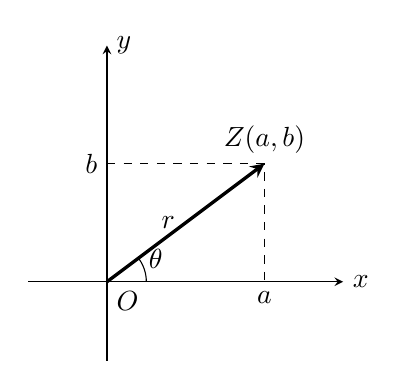
\begin{tikzpicture}[>=stealth]
\draw[->](-1,0)--(3,0)node[right]{$x$};
\draw[->](0,-1)--(0,3)node[right]{$y$};
\draw[dashed](0,1.5)node[left]{$b$}--(2,1.5)node[above]{$Z(a,b)$}--(2,0)node[below]{$a$};
\draw[very thick,->](0,0)--node[left]{$r$}(2,1.5);
\draw(.5,0) arc (0:35:.5)node[right]{$\theta$};
\node[below right]{$O$};
\end{tikzpicture}
    \caption{}
\end{figure}

显然
\[r=|z|=|a+bi|=\sqrt{a^2+b^2}\ge 0\]

特别地,当$b=0$时,$z$是一个实数,这时
\[r=|z|=|a|\qquad  \text{(与实数的绝对值概念一致)
}\]

又以实轴$OX$的正半轴为始边,向量$\VEC{OZ}$所在的射线为终边的角$\theta$,叫做复数$z=a+bi$的\textbf{幅角}.

由于任一不等于零的复数,按以上规定可有无限多个幅
角(终边相同的角)的值,因而,我们进一步约定:

满足$0<\theta<2\pi$的幅角$\theta$的值,叫做幅角的\textbf{主值},并记作$\arg z$,即$0\le \arg z<2\pi$. 
因此,任一非零复数$z$的幅角$\theta=\arg z+2k\pi\; (k\in\Z)$

这样一来,每一个不等于零的复数,就只有唯一的模与唯一的幅角主值,并可被它的模与幅角主值所唯一确定。

应该指出,由于复数$z=0$对应于复平面上的零向量(一个点),而且零向量的方向是任意的,因此,复数$z=0$的模$|z|=0$,它的幅角却是任意的。

\begin{example}
试比较复数$z_1=1+\sqrt{2}i$,$z_2=-\frac{1}{2}-i$的模的大小.
\end{example}

\begin{solution}
$\because\quad |z_1|=\sqrt{1+2}=\sqrt{3},\quad |z_2|=\sqrt{\frac{1}{4}+1}=\frac{1}{2}\sqrt{5},\qquad \sqrt{3}>\frac{1}{2}\sqrt{5}$

$\therefore\quad |z_1|>|z_2|$.
\end{solution}

一般来说,两个复数中,至少有一个不是实数,就不能比较它们的大小,但任意两个复数的模,总是可以比较大小的.

\begin{example}
    如果$a$,$b$都是正实数,试求:
\begin{multicols}{4}
\begin{enumerate}[(1)]
    \item $\arg a$
    \item $\arg (-a)$
    \item $\arg (bi)$
    \item $\arg (-bi)$
\end{enumerate}
\end{multicols}
\end{example}

\begin{solution}
由于$a$,$b$是正实数,因此:
复数$a$,$-a$分别对应着复平面中正、负半实轴上的点(不包含原点). 所以
\begin{multicols}{2}
    \begin{enumerate}[(1)]
        \item $\arg (a)=0$
        \item $\arg (-a)=\pi$
    \end{enumerate}
    \end{multicols}
复数$bi$,$-bi$分别对应着复平面中正、负半虚轴上的点(不包含原点). 所以
\begin{multicols}{2}
    \begin{enumerate}[(1)]\setcounter{enumi}{2}
        \item $\arg (bi)=\frac{\pi}{2}$
        \item $\arg (-bi)=\frac{3\pi}{2}$
    \end{enumerate}
    \end{multicols}
\end{solution}

\begin{example}
    设$z\in\mathbb{C}$,试说明满足下列条件的点Z的集合组成什么样的图形?
\begin{multicols}{2}
\begin{enumerate}[(1)]
    \item $|z|=a$
    \item $2<|z|\le 4$
\end{enumerate}
\end{multicols}
\end{example}

\begin{solution}
\begin{enumerate}[(1)]
    \item 复数$z$的模等于$a\ge 0$,就是说它对应于复平面上的向量$\VEC{OZ}$的长度为$a$,也就是说它对应于复平面上的点$Z$到原点的距离为$a$. 所以,满足条件$|z|=a$的点的集合,当$a>0$时组成一个以$O$为圆心、以$a$为半径的圆;当$a=0$时,就是一个点(原点)。
\item 先将条件$2<|z|\le 4$化为$\begin{cases}
    |z|>2\\ |z|\le 4
\end{cases}$

\begin{minipage}{.45\textwidth}
 再分别考虑:满足$|z|>2$的点集组成圆$|z|=2$的外部;满足$|z|\le 4$的点集组成圆$|z|=4$的内部(包含边界)。同时满足以上两条件的点集,就是已求两集合的交集,也就是所要求的集合.

因此,满足$2<|z|\le 4$的点的集合是以$O$为圆心,以2及4为半径的两图所夹的圆环,其中包含外边界,但不包括内边界(图1.4).   
\end{minipage}\hfill
\begin{minipage}{.45\textwidth}
    \centering
\begin{tikzpicture}[>=stealth, scale=.4]

\draw[ thick, pattern=north east lines](0,0) circle (4);
\fill[color=white](0,0) circle (2);    
\draw[dashed,  thick](0,0) circle (2);    
\draw[->](-6,0)--(6,0)node[right]{$x$};
\draw[->](0,-6)--(0,6)node[right]{$y$};
\node [below right]{$O$};
\node at (2,0)[below right]{2};
\node at (4,0)[below right]{4};
\node at (0,2)[below right]{2};
\node at (0,4)[above right]{4};

\end{tikzpicture}
    \captionof{figure}{ }
\end{minipage}

\end{enumerate}    
\end{solution}

\begin{ex}
\begin{enumerate}
    \item 求出下列复数的模,并按其大小用不等号连起来:
\[\sqrt{2}-i,\quad -2+i,\quad 7,\quad 2i,\quad -1-i\]
  \item   设$|z|=r$, $\arg z=a$,试求出$|\bar z|$, $\arg \bar z$.
  \item 求证:复数$z_1=-3i$, $z_2=\sqrt{2}+\sqrt{7}i$, $z_3=\sqrt{7}-\sqrt{2}i$, $z_4=-2+\sqrt{5}i$所对应的四个点共圆,并写出个这圆周上的所有点应满足的条件.
\item   你能指出满足下列条件的复数所对应的点集组成什么图形吗?
\begin{multicols}{2}
\begin{enumerate}[(1)]
    \item $\arg z=\frac{\pi}{4}$
    \item $\frac{\pi}{4}\le \arg z\le \frac{\pi}{2}$
\end{enumerate}
\end{multicols}
\end{enumerate}

\end{ex}

\subsection*{习题1.1}
\begin{enumerate}
    \item 设复数$z= (a^{2}- 2a- 3 )+( a^{2}+ 2a- 3) i$, $a\in \mathbb{R} $, 
试问在什么条件下,这一复数是
\begin{multicols}{4}
\begin{enumerate}[(1)]
    \item 实 数 ?
    \item 零?
    \item 虚数?
    \item 纯虚数?
\end{enumerate}
\end{multicols}

\item 实数$a,b$取何值时,才能使复数$z_1=z_2$:
\begin{enumerate}[(1)]
    \item $z_{1}= \left(\frac{1}{2}a+ b \right)+\left( 5a+\frac{2}{3}b \right) i,\quad z_{2}= - 4+ 16i$ ;
    \item $z_{1}=(a+b)+24i,\quad z_{2}=-(5+abi)$;
    \item $z_{1}=8+2abi,\quad z_{2}=6i+a^{2}-b^{2}$;
    \item $z_{1}=2a^{2}-5a+2,\quad z_{2}=(b^{2}+b-2)i$;
    \item $z_{1}= 0,\quad z_{2}= (a- 1)^{2}+ (b^{2}+ 2b)i$.
\end{enumerate}
\item 求出下列各复数的共轭复数,并在复平面上描出表示这些互为共轭复数的点。
\[1- i, \quad - 2+ \sqrt {2}i, \quad - \sqrt {3}i, \quad 2, \quad i, \quad \sqrt {3}+ i\]
\item 求出上题中各复数的模及幅角的主值(可用反三角函数表示).
\item 实数$x,y$取何值时,才能使$z_1=\bar z_2$:
\begin{enumerate}[(1)]
    \item $z_{1}=( x-y )+5i,\quad  z_{2}=1-( 2x+y ) i$;
    \item $z_{1}=xy-( x+y)i,\quad  z_{2}=5+24 i$; 
    \item $z_{1}=( x^{2}-3x-2 )+( y^{2}-5y-6 ) i,\quad z_{2}=2$;
    \item $z_1=0,\quad z_2=(2x^2-5x+2)+i(y^2+y-2)$.
\end{enumerate}


\item 求证:两个复数互为共轭的必要条件是这两个复数
的模相等。
\item  在下列各题中,要使等式$| z_1|=2| z_2|$成立,试
求实数$x,y$的值:
\begin{enumerate}[(1)]
    \item $z_{1}=x-1-2i,\quad  z_{2}=1+( x+1 )i$;
    \item $z_{1}=( x-y+1 )+2 ( x+y-3 )i,\quad z_{2}=\frac{x-y+1}{2\sqrt{2}}i $
\end{enumerate}

\item  设$a,b\in\mathbb{R}$, 它们取何值时,表示复数$z=(a-b-1)+(2a-b-5)i$在复平面上的点,才能在$y=x$直线上?
\item 试求满足下列条件的复数$x+yi$在复平面上对应的点
的轨迹:
\begin{multicols}{3}
\begin{enumerate}[(1)]
    \item $|x+yi|=3$
    \item $|x+yi|<3$
    \item $|x+yi|\ge 3$
    \item $2\le |x+yi|\le 3$
    \item $0<|x+yi|<3$
\end{enumerate}
\end{multicols}
\item 设$z=a+bi,\; a,b\in\mathbb{R}$. 问:满足下列条件的点
$Z(a,b)$的集合组成什么图形?
\begin{multicols}{2}
\begin{enumerate}[(1)]
    \item $0\le |a|<1$
    \item $a>0,\; b>0,\quad a^2+b^2>4$
\end{enumerate}
\end{multicols}

\item 想想看:若已知一个非零复 数$z=a+bi$, 你能求
出它的幅角来吗?它的主值又如何求出?举例说明。

\item 满足条件$\frac{\pi}{6}\le \arg z\le \frac{\pi}{2}$的复数,在复平面上对应着什么样的点集?

\end{enumerate}

\section{复数的四则运算}
本节讨论复数的四则运算,我们将根据引进的新数——虚数单位$i$的特征$i^2=-1$和希望它遵从“数系运算通性”的要求,合理地提出运算法则,并进一步应用这些法则,有效地进行运算,同时,根据复数的几何意义,我们将相应地给出复数运算的几何意义.

\subsection{复数的加、减法}
\subsubsection{加法}
复数的加法运算按照以下规定的法则进行:设$z_1=a+bi$, $z_2=c+di$是任意两个复数,则
\[z_1+z_2=(a+bi)+(c+di)=(a+c)+(b+d)i\]

可见,任意两个复数的和仍然是一个复数.

特别地,根据这一规定我们可求出任一个实数$a$和任一纯虚数$bi$的和:
\[(a+0i)+(0+bi)=(a+0)+(0+b)i=a+bi\]

由此可知,复数$a+bi$,既可认定为一个数,又可认定它为实数$a$与纯虚数$bi$的和,今后,对于表达复数$a+bi$中的“$+$”号与表达加法运算的“$+$”号,我们将认为是一样的。

不难验证,复数加法法则的规定满足“运算通性”。
即 : 设 $z_1, z_2, z_3\in \mathbb{C}$, 则
\begin{align}
    z_{1}+ z_2 &= z_{2}+ z_{1}\tag{交换律成立}\\
    z_{1}+\left( z_{2}+z_{3} \right)&=\left( z_{1}+z_{2} \right)+z_{3}=z_{1}+z_{2}+z_{3}\tag{结合律成立}\\
    z_{1}+ 0&= 0+ z_{1}= z_{1}\tag{零的运算特性保持}
\end{align}

\begin{example}
    试求下列复数的和:
\begin{enumerate}[(1)]
    \item $(5-3i)+(-\sqrt{2}+i)$
    \item $( 9+ 6i) + ( 9- 6i)$
    \item $( 1- i) + ( - 1+ 2i) + 7+ \sqrt {2}i$
\end{enumerate}
\end{example}

\begin{solution}
\begin{enumerate}[(1)]
    \item $( 5- 3i) + ( - \sqrt {2}+ i) = 5- \sqrt {2}$
    \item $( 9+ 6i) + ( 9- 6i) = 18+ 0i= 18$
    \item $( 1- i) + ( - 1+ 2i) +7+ \sqrt {2}i=(1-1+7)+(-1+2+\sqrt{2})i=7+(1+\sqrt{2})i$
\end{enumerate}
\end{solution}


由于复数可以用复平面上的“位置”向量来表示,因此,复数加法的几何意义就是:复数的加法可以按照向量的“平行四边形”法则来进行,即,先将求和的两个复数所对应的向量$\overrightarrow{OZ_{1}}$, $\overrightarrow{OZ_{2}}$画出,若这两个向量不共线,再以这两个向量为邻边作平行四边形$OZ_1ZZ_2$, 则这个平行 四 边形的对角线$OZ$所示的向量$\overrightarrow{OZ}$, 就 对 应 着 已 知 两 个 复 数 的 和(如图1.5).

\begin{figure}[htp]
    \centering
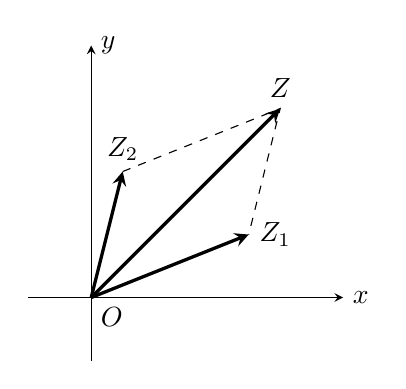
\begin{tikzpicture}[>=stealth, scale=.8]
\draw[->](-1,0)--(4,0)node[right]{$x$};
\draw[->](0,-1)--(0,4)node[right]{$y$};
\node [below right]{$O$};
\draw[very thick, ->](0,0)--(.5,2)node[above]{$Z_2$};
\draw[very thick, ->](0,0)--(2.5,1)node[right]{$Z_1$};
\draw[very thick, ->](0,0)--(3,3)node[above]{$Z$};
\draw[dashed](.5,2)--(3,3)--(2.5,1);


\end{tikzpicture}
    \caption{}
\end{figure}

$\overrightarrow{OZ_{1}}$ 与$\overrightarrow{OZ_{2}}$共线,只要在$\overrightarrow{OZ_{1}}$的方向上紧接着延长一个$\overrightarrow{Z_{1}Z}$,使$\overrightarrow{Z_{1}Z}=\overrightarrow{OZ_{2}}$. 这时同样得到向量$\overrightarrow{OZ}$, 它对应着已识两复数的和(相当于作一个退缩成一条线段的平行四边形).

显然,两个共轭复数的和是一个实数,它对应着实轴上的一个向量. 

\subsubsection{减法}
复数的减法仍定义为加法
的逆运算,即:满足$(c+di)+(x+yi)=a+bi$的复数$x+yi$,就叫做复数$a+b$减去$c+di$的差,记作
\[x+yi=(a+bi)-(c+di)\]

根据复数加法法则和复数相等的定义,可以得出复数的减法法则
\[(a+bi)-(c+di)=(a-c)+(b-d)i\]

可见,两复数的差,仍是一个确定的复数,就是说,复数集对于减法也是封闭的.

同样,复数的减法的几何意义就是用向量减法的“三角
形法则”来表示,即:两个复数的差
$z_1-z_2$(向量$\VEC{OZ_1}-\VEC{OZ_2}$)与连结两个向量终点并
指向被减向量终点的向量对应
(图1.6),即
\[\VEC{OZ_1}-\VEC{OZ_2}=\VEC{Z_2Z_1}\]

\begin{figure}[htp]
    \centering
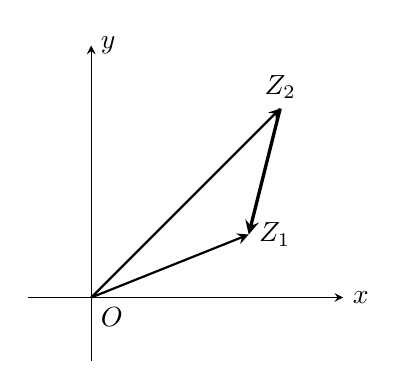
\begin{tikzpicture}[>=stealth, scale=.8]
\draw[->](-1,0)--(4,0)node[right]{$x$};
\draw[->](0,-1)--(0,4)node[right]{$y$};
\node [below right]{$O$};
\draw[ thick, ->](0,0)--(3,3)node[above]{$Z_2$};
\draw[ thick, ->](0,0)--(2.5,1)node[right]{$Z_1$};
\draw[very thick, ->](3,3)--(2.5,1);


\end{tikzpicture}
    \caption{}
\end{figure}

综上所述,复数的加、减法与我们熟悉的多项式加、减法是类似的,就是把复数的实部、虚部分别相加、减,即
\[(a+bi)\pm (c+di)=(a\pm c)+(b\pm d)\]

\begin{example}
    计算$(3-4i)+(-2+i)-(5+2i)$
\end{example}

\begin{solution}
 $$(3-4i)+(-2+i)-(5+2i)
=(3-2-5)+(-4+1-2)i=-4-5i.$$   
\end{solution}

\begin{example}
    设复数$z_1=a+bi$, $z_2=c+di$, 试求这两复数在复平面上所描述的两点之间的距离.
\end{example}

\begin{solution}
    由于$z_1$与$z_2$在复平面上所描述的两点$Z_1$, $Z_2$之间的距离$d$,就是向量$\VEC{Z_1Z_2}$的模,因而,只要求出向量$\VEC{Z_1Z_2}$所对应的复数,并求出它的模即可。

    $\because\quad \VEC{Z_1Z_2}=\VEC{OZ_2}-\VEC{OZ_1}$

$\therefore\quad \VEC{Z_1Z_2}$对应于复数$z_2-z_1$,于是
\[\begin{split}
d&=|\VEC{Z_1Z_2}|=|z_2-z_1|\\
&=|(c+di)-(a+bi)|=|(c-a)+(d-b)i|\\
&=\sqrt{(c-a)^2+(d-b)^2}    
\end{split}\]
\end{solution}

\begin{example}
    根据复数的几何意义及向量表示,试求复平面内以$P(a,b)$点为圆心,$r$为半径的圆的方程.
\end{example}

\begin{figure}[htp]
    \centering
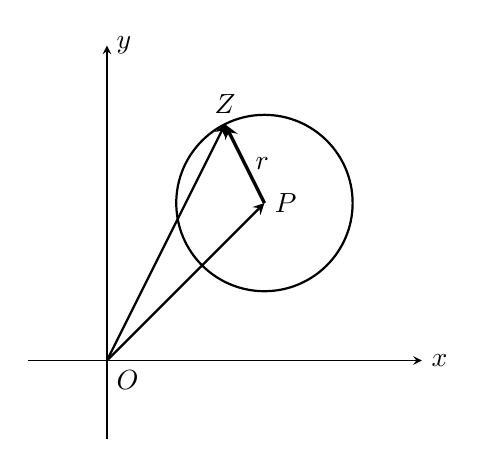
\begin{tikzpicture}[>=stealth, scale=1]
\draw[->](-1,0)--(4,0)node[right]{$x$};
\draw[->](0,-1)--(0,4)node[right]{$y$};
\node [below right]{$O$};
\draw[ thick, ->](0,0)--(1.5,3)node[above]{$Z$};
\draw[ thick, ->](0,0)--(2,2)node[right]{$P$};
\draw[thick](2,2)circle(1.12);
\draw[->, very thick](2,2)--node[right]{$r$}(1.5,3);

\end{tikzpicture}
    \caption{}
\end{figure}


\begin{solution}
    设圆心$P(a,b)$与复数$p=a+bi$对应,圆上任一点$Z(x,y)$与复数$z=x+yi$对应,由于已知圆的半径为$r$,因
此,向量$\VEC{PZ}$的模就是定长$r$. 即
$|\VEC{PZ}|=r$.

又由于$\VEC{PZ}=\VEC{OZ}-\VEC{OP}$,因而向量$\VEC{PZ}$就对应着复数$z-p=(x+yi)-(a+bi)=(x-a)+(y-b)i$.

所以,圆上任一点$Z$应满足$|\VEC{PZ}|=|\VEC{OZ}-\VEC{OP}|=r$,即
\[|z-p|=r\]
这就是复平面上以$P$为圆心,$r$为半径的圆的方程.

若进一步求出$|z-p|=|(x-a)+(y-b)i|
=\sqrt{(x-a)^2+(y-b)^2}$
代入圆方程,并化简。就得出用实数表示的圆的一般方程:
\[(x-a)^2+(y-b)^2=r^2\]
特别地,当$P$点在原点时,圆的方程就变成为
$$|z|=r$$
或
$$x^2+y^2=r^2$$
\end{solution}

\begin{ex}
\begin{enumerate}
    \item 利用复数加法法则和实数、虚数单位运算通性,验证:复数加法的交换律和结合律都成立.
    \item 计算(分别求和,再求差):
\begin{multicols}{2}
\begin{enumerate}[(1)]
    \item $(2+3i)\pm (1+i)$
    \item $(2+4i)\pm (1-i)$
    \item $(-3i-2)\pm (-1-i)$
    \item $-2i\pm (-4+i)$
    \item $(2-3i)\pm (-5i)\pm(-1+7i)$
\end{enumerate}
\end{multicols}
\item 将上题中的各小题,用向量法求和.
\item 求证:两个互为共轭的复数之和为实数;两互为共轭的复数之差为纯虚数或零.
\item 想想看:在复平面上,以$P(a,b)$为圆心、以r为半径的圆内所有点的集合,可用什么样的条件给定?
\end{enumerate}
\end{ex}

\subsection{复数的乘、除法}
\subsubsection{乘法}
复数的乘法运算按照以下规定的法则进行:设$z_1=a+bi$, $z_2=c+di$是任意两复数,则
\[z_1\cdot z_2=(a+bi)\cdot (c+di)=(ac-bd)+(ad+bc)i\]
其中,由于我们要求乘法运算仍应保持“运算通性”,因而,这一规定说明复数的乘法与多项式乘法是类似的,只要将结果中的$i^2$换成$-1$,分别合并实部与虚部即可.

可见,任意两个复数的乘积仍然是一个复数,也就是说,复数集对于乘法也是封闭的.

特别地,根据这一规定,对两个互为共轭复数$z$与$\bar z$,我们有
\[z\cdot \bar z=(x+yi)\cdot (x-yi)=x^2+y^2\]

因此,互为共轭的两复数之积是一个实数,它等于每一复数的模的平方,即
\[z\cdot \bar z=|z|^2=|\bar z|^2\]

容易验证,复数乘法运算也具有“数系运算通性”,即对于任意$z_1,z_2,z_3\in\mathbb{C}$,都有
\begin{align}
z_1\cdot z_2  &= z_2\cdot z_1 \tag{乘法交换律成立}\\
z_1\cdot (z_2\cdot z_3)  &= (z_1\cdot z_2)\cdot z_3=z_1\cdot z_2\cdot z_3 \tag{乘法结合律成立}\\
z_1\cdot (z_2+ z_3)  &= z_1\cdot z_2+ z_1\cdot z_3 \tag{乘法对加法的分配律成立}\\
z_1\cdot 0  &= 0\cdot z_1=0 \tag{零的运算特性保持}\\
z_1\cdot 1  &= 1\cdot z_1=z_1 \tag{1的运算特性保持}
\end{align}

还应该指出,复数乘方运算、幂的概念与实数完全相同,而且由于复数的乘法满足交换律、结合律,所以在实数集$\R$中的指数运算律,在复数集$\mathbb{C}$中仍然成立,即

对任意$z_1,z_2,z\in\mathbb{C}$及$m,n\in\N$, 都有
\[\begin{split}
    z^m\cdot z^n&=z^{m+n}\\
    (z^m)^n&=z^{m\cdot n}\\
    (z_1\cdot z_2)^n&=z^{n}_1\cdot z^{n}_2\\
\end{split}\]

这样,我们由定义$i^2=-1$,运用指数运算律可以得出:
\[\begin{split}
i^3&=i\cdot i^2=-i\\
i^4&=i^2\cdot i^2=(-1)\cdot (-1)=1\\
i^5&=i^4\cdot i=i\\
\cdots&\cdots
\end{split}\]

一般地,对任意$n\in\mathbb{N}$,我们可归纳出:
\[\begin{split}
    i^{4n}&=(i^4)^n=1^n=1\\
    i^{4n+1}&=(i^4)^n\cdot i=i\\
    i^{4n+2}&=(i^4)^n\cdot i^2=-1\\
    i^{4n+3}&=(i^4)^n\cdot i^3=-i\\
\end{split}\]
即,对于数$n\in\N$,则
\[i^{4n}=1,\qquad i^{4n+1}=i,\qquad i^{4n+2}=-1,\qquad i^{4n+3}=-i\]

\begin{example}
    计算$(5-4i)(1-i)(-2+3i)$.
\end{example}

\begin{solution}
\[(5-4i)(1-i)(-2+3i)=(1- 9i) (- 2+ 3i) = 25+ 21i\]
\end{solution}

\begin{example}
    计算$\left(-\frac12+\frac{\sqrt{3}}{2}i\right)^6$
\end{example}

\begin{solution}
\[\begin{split}
    \left(-\frac12+\frac{\sqrt{3}}{2}i\right)^6&=\left[\left(-\frac12+\frac{\sqrt{3}}{2}i\right)^2\right]^3\\
&= \left(\frac{1}{4}-\frac{\sqrt{3}}{2}i+\frac{3i^{2}}{4}\right)^{3}=\left(-\frac{1}{2}-\frac{\sqrt{3}}{2}i\right)^3\\
&=\left( - \frac 12\right) ^{3}- 3\left( \frac {- 1}{2}\right)^{2}\cdot \frac {\sqrt {3}}2i+3\left(-\frac{1}{2}\right)\left(\frac{\sqrt{3}}{2}i\right)^{2}-\left(\frac{\sqrt{3}}{2}i\right)^{3}\\
&=-\frac{1}{8}-\frac{3\sqrt{3}}{8}i+\frac{9}{8}+\frac{3\sqrt{3}}{8}i=1
\end{split}\]
\end{solution}


\subsubsection{除法}

复数的除法同样定义为乘法的逆运算,即:满足$(c+di)(x+yi)=a+bi\; (c+di\neq0)$的复数$x+yi$叫做复数$a+bi$除以$c+di$的商,记作
$$x+yi=\frac{a+bi}{c+di}\quad \text{或}\quad( a+bi )\div( c+di ) $$

根据两个共轭复数的乘积是一个实数以及乘法运算法
则,可以得出复数的除法法则:

当$c+ di\neq 0$ 时,
\[\frac{a+bi}{c+di}=\frac{(a+bi)(c-di)}{(c+di)(c-di)}=\frac{ac+bd}{c^2+d^2}+\frac{bc-ad}{c^2+d^2}i\]
其中由于$c+di\ne 0$,因而$c$、$d$不同时为零,所以,$c^2+d^2\ne 0$.可见这样求得的商是唯一确定的一个复数,也就是说,复数集$\mathbb{C}$对于除法(除数不为零)也是封闭的.

\begin{example}
    计算$(2-3i)\div (-3+4i)$
\end{example}

\begin{solution}
\[\begin{split}
    (2-3i)\div (-3+4i)&=\frac{2-3i}{-3+4i}=\frac{(2-3i)(-3-4i)}{(-3+4i)(-3-4i)}\\
    &=\frac{-18+i}{25}=-\frac{18}{25}+\frac{1}{25}i
\end{split}\]
\end{solution}

可以看出,复数乘、除法法则的公式并不需要硬记,乘法类似于多项式乘法,除法可视为分式的分子、分母同乘以除数的共轭数,并注意正确应用运算通性及$i^2=-1$,就可得出结果.

\begin{ex}
\begin{enumerate}
    \item 验证复数乘法对于加法满足分配律.
    \item 计算下列各式:
\begin{multicols}{2}
\begin{enumerate}[(1)]
\item $(4-3i)(-\sqrt{3}i)$
\item $\left(\frac{1}{2}-\frac{\sqrt{3}}{2}i\right)(1+i)$
\item $\left(\frac{1}{2}-\frac{\sqrt{3}}{2}i\right)^3\cdot \left(\frac{1}{2}+\frac{\sqrt{3}}{2}i\right)^3$
\item $(-\sqrt{77}+\sqrt{112}i)\cdot 0$
\end{enumerate}
\end{multicols}

\item  (口答)计算:
\[i^{13},\quad i^{22},\quad i^{36},\quad i^{43},\quad i^{70},\quad i^{101},\quad i^{355},\quad i^{404} \]
\[\frac{1}{i},\quad \frac{1}{i^2},\quad \frac{1}{i^3},\quad \frac{1}{i^4},\quad \frac{1}{i^{11}}\]
\item     计算:
\begin{multicols}{3}
\begin{enumerate}[(1)]
    \item $\frac{1}{1+i}$
    \item $\frac{1}{\sqrt{2}i}$
    \item $\frac{2i}{1-i}$
    \item $\frac{2+i}{7+4i}$
    \item $\frac{1}{(9+2i)^2}$
    \item $\frac{(1-i)^2}{(1+i)^3}$
\end{enumerate}
\end{multicols}
\end{enumerate}
\end{ex}

\subsection{复数集内的多项式与方程}
我们已经学习过实数范围内的多项式,而且明确多项式的元(未知数)只要求它满足“运算通性”,因此,对于复系数的多项式运算或未知数(元)取复数值的多项式求值,都可以与实系数多项式同样处理.

\begin{enumerate}
    \item 复系数多项式的四则运算举例
    
例如$f(x)=x+i$, $g(x)=2x+1-i$,则
\[\begin{split}
f(x)+g(x)&=3x+1\\
f(x)-g(x)&=-x-1+2i\\
f(x)\cdot g(x)&=2x^2+(1+i)x+(1+i)\\
g(x)&=2\cdot f(x)+1-3i    
\end{split}\]
这就是说,$g(x)$除
以$f(x)$可得商2,余$1-3i$(由综合除法得).

\item 多项式求值举例

例如$f(x)=x^2+x+1$,
则
\[\begin{split}
  f(i)&=i^2+i+1=i\\
f(1+i)&=(1+i)^2+(1+i)+1=2+3i.  
\end{split}\]

\item 复系数多项式的因式分解举例

例如:在复数范围内,$f(x)=x^2+1$可以进一步分解
\[x^2+1=x^2-(-1)=x^2-i^2=(x+i)(x-i)\]

\item 复数范围内的方程与方程组,均可按实数范围时的方法求解

\item 由带余除法导出的多项式的余式定理,对于复系数
的多项式仍然适用. 例如
$f(x)=x^4+2x^3-3x^2+5$除以$x-2i$所得的余式为:
\[R=f(2i)=(2i)^4+2(2i)^3-3(2i)^2+5
=33-16i\]
\end{enumerate}

\begin{example}
    在复数范围内分解因式$x^4-16$
\end{example}

\begin{solution}
\[x^{4}-16=(x^{2}-4)(x^{2}+4)=(x- 2) (x+ 2) (x- 2i) (x+ 2i)\]
\end{solution}

\begin{example}
    解方程$x^2-6x+10=0$
\end{example}

\begin{solution}
    利用求根公式,得
$$x=\frac{6\pm\sqrt{36-40}}{2}=\frac{6\pm\sqrt{-4}}{2}=3\pm i$$
$\therefore\quad x_{1}= 3+ i,\quad x_{2}= 3- i$
\end{solution}

\begin{example}
     解方程
$\begin{cases}
    2x+(1+i)y=6-2i\\
    (3-i)x+2i y=13-i
\end{cases}$
\end{example}

\begin{solution}
   用行列式法解,由于
\[\begin{split}
    \Delta&=\begin{vmatrix}
    2& 1+i\\
    3-i& 2i
\end{vmatrix}=4i-(1+i)(3-i)=-4+2i\\
\Delta_{1}&=\begin{vmatrix}
   6- 2i& 1+i\\
    13-i& 2i
\end{vmatrix}=-10\\
\Delta_{2}&=\begin{vmatrix}
    2& 6-2i\\
     3-i& 13-i
 \end{vmatrix}=10+10i\\
\end{split}\]
$\therefore\quad x= \frac {\Delta_{1}}{\Delta} = - \frac {- 10}{- 4+ 2i}= 2+ i,\quad 
y=\frac{\Delta_{2}}{\Delta}=\frac{10+10i}{-4+2i}=-1-3i$

因此,方程组的解集为$\{(x,\; y)\}=\{(2+i,\;  -1-3i)\}$.
\end{solution}

\begin{ex}
\begin{enumerate}
    \item 已知$f(x)=2x^2+(1+i)x+(1-i)$,试求$f(i)$, $f(-i)$, $f(1+i)$和$f(0)$的值.
    \item 在复数范围内分解因式$2x^4-5x^2-3$.
    \item 解方程组$\begin{cases}
        ix-y=2(i-1)\\
        x-iy=0
    \end{cases}$
\end{enumerate}
\end{ex}

\subsection*{习题1.2}

\begin{enumerate}
    \item 计算:
\begin{enumerate}[(1)]
    \item $\left(\frac{2}{3}+i\right)+\left(1-\frac{2}{3}i\right)-\left(\frac{1}{2}+\frac{3}{4}i\right)$
    \item $[(a+b)+(a-b)i]-[(a-b)-(a+b)i]$
\end{enumerate}

\item 设复数$z_1=3+2i$, $z_2=-2+5i$在复平面上分别对应着点$Z_1,Z_2$. 试求向量$\VEC{Z_1Z_2}$与$\VEC{Z_2Z_1}$所表示的复数.
\item 试求复平面上点$P(2,1)$与点$Q(3,-1)$之间的距离.
\item 求证:两个复数和的共轭复数,等于这两个复数的共轭复数之和.
\item 设$z_1,z_2$是非零复数,用几何方法证明:
\begin{enumerate}[(1)]
    \item $\big||z_1|-|z_2|\big|\le |z_1\pm z_2|\le |z_1|+|z_2|$
    \item $|z_1+z_2|^2+|z_1-z_2|^2=2|z_1|^2+2|z_2|^2$
\end{enumerate}
\item  写出复平面内任意两点连线段的垂直平分线的方程。
\item  设复平面内有两定点$F_1(-\sqrt{5},0)$, $F_2(\sqrt{5},0)$,试求到这两定点的距离之和等于6的点的轨迹方程(椭圆方程).
\item  计算:
\begin{enumerate}[(1)]
    \item $(\sqrt{a}+\sqrt{b}i)(\sqrt{a}-\sqrt{b}i)\quad (a,b\in\mathbb{R})$
    \item $(1-2i)(-0.2+0.3i)(0.5-0.4i)$
    \item $(1+i)+(2-i^{3})+(3-i^{5})+(4-i^{7})$
    \item $(\sqrt{2}-\sqrt{2}i)^{2}\cdot\left(\frac{1}{4}+\frac{1}{4}i\right)$
    \item $(a+bi)^{3}+(a-bi)^{3}$
    \item $\begin{vmatrix}
        1-i&i\\1+i&-i
    \end{vmatrix}+\begin{vmatrix}
        i&1&0\\1&2i&1\\0&1&3i
    \end{vmatrix}$
\end{enumerate}

\item 利用公式$(a+bi)(a-bi)=a^2+b^2$, 把下列各式分解因式:
\begin{multicols}{2}
 \begin{enumerate}[(1)]
    \item $a^{4}-b^{4}$
    \item $x^{2}+2x+3$
    \item $a^{2}+2ab+b^{2}+c^{2}$
    \item $x^{3}-2x+4$
\end{enumerate}   
\end{multicols}


\item 设$\omega = - \frac 12+ \frac {\sqrt {3}}2i$, 求证:
\begin{enumerate}[(1)]
    \item $1+\omega+\omega^{2}=0$
    \item $\omega^{3}=1$
    \item $a^{3}+b^{3}+c^{3}-3abc=(a+b+c)(a+\omega b+\omega^{2}c)(a+\omega^{2}b+\omega c)$
\end{enumerate}
\item 计算:
\begin{multicols}{2}
\begin{enumerate}[(1)]
    \item $\frac{1}{2-4i}$
    \item $\frac{3-2i}{1+i}$
    \item $\frac{1+i}{(1-i)^{2}}$
    \item $\frac{1+2i}{2-i^3}$
    \item $\frac{(1-2i)^2}{3-4i}-\frac{(2+i)^2}{4-3i}$
    \item $\frac{\sqrt{3}-\sqrt{2}i}{\sqrt{3}+\sqrt{2}i}-\frac{\sqrt{2}+\sqrt{3}i}{\sqrt{2}-\sqrt{3}i}$
\end{enumerate}
\end{multicols}

\item 若$z_1,z_2\in\mathbb{C}$, 且$z_1\cdot z_2=0$, 则$z_1,z_2$中至少有一个等于0.

\item 已知$\frac1z=\frac{1}{z_{1}}+\frac{1}{z_{2}}$, 且$z_1=2+3i$, $z_{2}=1-i$,
求$z$.

\item 已知$z^2=5-12i$, 求$z$.

\item 证明下列各命题:
\begin{enumerate}[(1)]
    \item 作两个复数的和、差、积、商(除数不为零)的
共轭复数,分别等于这两个复数的共轭复数的和、差、积、商.
\item 若$f(x)$是一个一元多项式,则对于任意复数
$z$, 有$\overline{f(z)}=f(\bar{z})$.
\end{enumerate}

\item 已知$f(z)=\frac{z^2-z+1}{z^2+z+1}$, 求$f(2+3i)$, $f(1-i)$的值.

\item  如果规定$i^0=1$, $i^{-m}=\frac{1}{i^m}\; (m\in\mathbb{N})$, 证明:对一切整数$n$,以下等式成立:
$$i^{4n}={1},\quad i^{4{n+1}}=i,\quad  i^{4{n+2}}=-1,\quad  i^{4n+3}=-i.$$
\item 根据$i^2=-1$及要求复数运算满足“通性”,试说
明复 数 加 法 、 乘 法 法 则 规 定 是 合 理 的。

\item 怎样的复数$z$, 才能满足条件:
\begin{multicols}{2}
\begin{enumerate}[(1)]
    \item $\overline {z}= z$
    \item $\overline {z}= -z$
    \item $z\cdot \bar z=[{\rm Re}(z)]^2$
    \item $z-\bar z=2[{\rm Im}(z)]$
\end{enumerate}    
\end{multicols}

\item 应用余式定理,求下列各余式;
\begin{enumerate}[(1)]
    \item $f( x) = x^{4}- 3x^{3}+ 2x^{2}- x+ i$
除以$g(x)=x+i$
\item $f( x) = x^{4}- 3x^{3}+ 2x^{2}- x+ i$
除以$h(x)=(1+i)x-1+i$
\end{enumerate}
\item 应用综合除法,将多项式
$f\left(x\right)=x^{3}+3\left({1+i}\right)x^{2}-2(5-3i)x-4\left(1+2i\right)$
展开成$(x+i)$的幂的代数和形式.

\item 解方程组$\begin{cases}
    x_1+2x_2=1+i\\
    ix_2+x_3=2i\\
    ix_1-ix_3=1-i
\end{cases}$
\end{enumerate}

\section{复数的三角形式}

我们已经建立了复数集
\[\mathbb{C}=\{x+yi\mid x,y\in\R,\; i^2=-1\}\]
与复平面上的点集以及复平面上的全体向量(由原点出发)集合间的一一对应关系,并且明确了复数的模与幅角、幅角的主值等概念,这一节我们将学习复数的另一种表达形式. 就是由它的模与幅角所确定的三角形式,这将有助于复数乘法、除法、乘方、开方运算的进一步简便。

\subsection{复数的三角形式}

设$z=a+bi,\; (a,b\in\R)$,对应着复平面上的向量$\VEC{OZ}$(图1.8),并设它的模$|\VEC{OZ}|=r$,幅角为$\theta$. 若$z=a+bi\ne 0$,则可得
\[a=r\cdot \cos\theta,\qquad b=r\cdot \sin\theta\]
\begin{figure}[htp]
    \centering
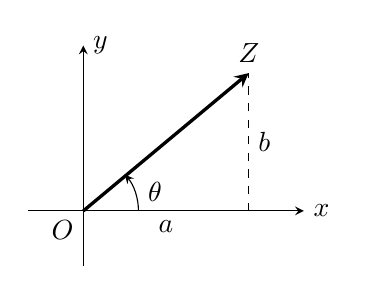
\begin{tikzpicture}[>=stealth, scale=.7]
\draw[->](-1,0)--(4,0)node[right]{$x$};
\draw[->](0,-1)--(0,3)node[right]{$y$};
\node[below left]{$O$};
\draw[->, very thick](0,0)--(3,2.5)node[above]{$Z$};
\draw[dashed](3,0)--node[right]{$b$}(3,2.5);
\node at (1.5,0)[below]{$a$};
\draw[->](1,0)node[above right]{$\theta$} arc (0:41:1);
\end{tikzpicture}
    \caption{}
\end{figure}


$\therefore\quad z=a+bi=r\left(\pc{\theta}\right)$

因此,对于任何一个复数$z=a+bi$,都可以表示成
$r(\cos\theta +i\sin\theta)$
的形式(其中$r=\sqrt{a^2+b^2}$),并叫做这个复数的三角形式(也叫做复数的极坐标形式);为了方便,我们将$a+bi$叫做复数的代数形式.

复数的代数形式$z=a+bi$与三角形式$z=r(\cos\theta +i\sin\theta)$之间,由图1.8可知有下列互化的关系:
\[\begin{cases}
 a=r\cos\theta\\
b=r\sin\theta   
\end{cases},\qquad \begin{cases}
    r=\sqrt{a^2+b^2}\\ \tan\theta=b/a
\end{cases}\]
($\theta$只要取主值,且要考虑$a$,$b$的正负).

\begin{example}
 将下列复数的代数形式化为三角形式: 
\begin{multicols}{2}
\begin{enumerate}[(1)]
    \item $\sqrt{3}+i$
    \item $-\frac{1}{2}+\frac{\sqrt{3}}{2}i$
    \item $-1$
    \item $\cos\theta-i\sin\theta$
\end{enumerate}
\end{multicols}  
\end{example}

\begin{solution}
\begin{enumerate}[(1)]
    \item $r=\sqrt{3+1}=2$, $\tan\theta=\frac{1}{\sqrt{3}}=\frac{\sqrt{3}}{3}$,且$a,b$均为正值,$\theta$在I象限,因而$\arg(\sqrt{3}
    +i)=\frac{\pi}{6}$

    $\therefore\quad \sqrt{3}+i=2\left(\pc{\frac{\pi}{6}}\right)$
\item $r=\sqrt{\frac{1}{4}+\frac{3}{4}}=1$, $\tan\theta=-\sqrt{3}$,且$a<0, b>0$,$\theta$在II象限,因而$\theta=\frac{2\pi}{3}$(主值)

$\therefore\quad -\frac{1}{2}+\frac{\sqrt{3}}{2}i=\pc{\frac{2\pi}{3}}$

\item $r=1$, $\tan\theta =0$,且$a<0$,因此$\arg(-1)=\pi$

$\therefore\quad -1=\pc{\pi}$

\item $r=\sqrt{\cos^2\theta+\sin^2\theta}=1$

$\therefore\quad \cos\theta-i\sin\theta=\pcx{-\theta}=\pcx{2\pi-\theta}$

\end{enumerate}
\end{solution}


\begin{example}
    将下列复数的三角形式化为代数形式:
\begin{multicols}{2}
\begin{enumerate}[(1)]
    \item $2\left(\pc{\frac{\pi}{4}}\right)$
    \item $\sqrt{2}\left(\pc{\frac{5\pi}{6}}\right)$
    \item $\pc{101\pi}$
    \item $5\left(\pc{\frac{\pi}{2}}\right)$
\end{enumerate}    
\end{multicols}
\end{example}

\begin{solution}
\begin{enumerate}[(1)]
    \item $2\left(\pc{\frac{\pi}{4}}\right)=\sqrt{2}+\sqrt{2}i$
    \item $\sqrt{2}\left(\pc{\frac{5\pi}{6}}\right)=-\frac{\sqrt{6}}{2}+\frac{\sqrt{2}}{2}i$
    \item $\pc{101\pi}=\pc{\pi}=-1$
    \item $5\left(\pc{\frac{\pi}{2}}\right)=5i$
\end{enumerate}  
\end{solution}

\begin{rmk}
复数的三角形式$r(\pc{\theta})$中,必须满足
    $r>0$、式中保持“$+$”号两特征,至于幅角$\theta$则不一定非要取主值,除常用主值表示外,也可以在幅角中任取一个。例如,
\[\sqrt{2}-\sqrt{2}i=2\left[\pcx{-\frac{\pi}{4}}\right]\]
也是复数$\sqrt{2}-\sqrt{2}i$的三角形式.

此外,若$z=a+bi=0$,即$z=0+0i$,这时$r=0$,其幅角是任意实数,则$0=0(\pc{\theta})$.
\end{rmk}

\begin{ex}
\begin{enumerate}
    \item 判断下列给出的是不是复数的三角形式?若不是,请把它们化为三角形式:
\begin{multicols}{2}
    \begin{enumerate}[(1)]
        \item $2\left(\cos\frac{\pi}{4}-i\sin\frac{\pi}{4}\right)$
        \item $-2\left(\pc{\frac{\pi}{3}}\right)$
        \item $\frac{1}{2}\left(\pc{\frac{3\pi}{4}}\right)$
        \item $\cos\frac{7\pi}{5}+i\sin\left(-\frac{3\pi}{5}\right)$
    \end{enumerate}
\end{multicols}
    \item 将复数表示成三角形式:
\begin{multicols}{3}
    \begin{enumerate}[(1)]
        \item $2$
        \item $-3$
        \item $4i$
        \item $-2i$
        \item $1+i$
        \item $-4+3i$
        \item $-1-\sqrt{3}i$
        \item $\frac{\sqrt{3}}{2}-\frac{1}{2}i$
    \end{enumerate}
\end{multicols}
\item    写出下列复数的代数形式:
\begin{multicols}{2}
    \begin{enumerate}[(1)]
        \item $3\left(\pc{\frac{\pi}{3}}\right)$
        \item $\sqrt{2}\left(\pc{\frac{3\pi}{4}}\right)$
        \item $\frac{1}{\sqrt{3}}\left[\pcx{-\frac{\pi}{6}}\right]$
        \item $5\left(\pc{\frac{7\pi}{2}}\right)$
    \end{enumerate}
\end{multicols}

\item 想一想:“两个复数若相等,则它们的模与幅角必定相等”对吗?为什么?
\end{enumerate}
\end{ex}

\subsection{再谈复数的乘、除法和乘方运算}
通过第二节对复数四则运算的学习,我们会感到:复数的代数形式在进行加、减法运算时,步骤十分简明易学,但进行乘、除法和乘方运算时,却显得繁杂.

我们将会看到,复数的三角形式在进行乘、除、乘方甚至开方运算时,比代数形式要简捷得多.

\begin{blk}
 {定理1} 两个复数的乘积是一个复数,它的模等于两乘数的模的乘积;它的幅角等于两乘数的幅角的和,即   

设$z_1=r_1(\pc{\theta_1})$, $z_2=r_2(\pc{\theta_2})$,则
\[\begin{split}
z_1\cdot z_2 &=r_1(\pc{\theta_1})\cdot r_2(\pc{\theta_2})\\
&=r_1\cdot r_2 \left[\pcx{\theta_1+\theta_2}\right]
\end{split}\]
\end{blk}

\begin{proof}
\[\begin{split}
    \because\quad z_1\cdot z_2&=r_1\cdot r_2(\pc{\theta_1})(\pc{\theta_2})\\
&=r_1\cdot r_2 \left[\left(\cos\theta_1\cdot \cos\theta_2-\sin\theta_1\cdot \sin\theta_2\right)\right.\\
&\qquad \qquad +i\left.\left(\cos\theta_1\cdot \sin\theta_2+\sin\theta_1\cdot \cos\theta_2\right)\right]\\
&=r_1\cdot r_2 \left[\pcx{\theta_1+\theta_2}\right]
\end{split}\]

$\therefore\quad $定理成立.
\end{proof}

根据这一定理,联系复数的向量表示,我们可以给出两复数相乘的几何意义:

两复数$z_1=r_1(\pc{\theta_1})$与$z_2=r_2(\pc{\theta_2})$相乘时,可以先在复平
面上画出它们对应的向量$\VEC{OZ_1}$, $\VEC{OZ_2}$,然后将$\VEC{OZ_1}$旋转一个角$|\theta_2|$(若$\theta_2>0$时,就按逆时针方向旋转$\VEC{OZ_1}$;若$\theta_2<0$时,就按顺时针方向旋转$\VEC{OZ_1}$),再把它的模变为原来的$r_2$倍,就可得到向量$\VEC{OZ}$(图1.9所示),这一向量就对应着所求两复数的积.

\begin{figure}[htp]
    \centering
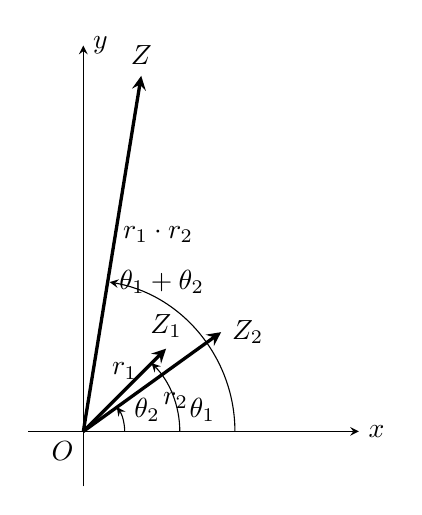
\begin{tikzpicture}[>=stealth, scale=.7]
\draw[->](-1,0)--(5,0)node[right]{$x$};
\draw[->](0,-1)--(0,7)node[right]{$y$};
\node[below left]{$O$};
\coordinate(Z1) at (1.5,1.5);
\coordinate(Z2) at (2.5,1.8);
\coordinate(Z) at (1.05,6.45);
\draw[->, very thick](0,0)--node[above]{$r_1$}(Z1)node[above]{$Z_1$};
\draw[->, very thick](0,0)--node[below right]{$r_2$}(Z2)node[right]{$Z_2$};
\draw[->, very thick](0,0)--node[above right]{$r_1\cdot r_2$}(Z)node[above]{$Z$};
\draw[->](.75,0)node[above right]{$\theta_2$}arc (0:36:.75);
\draw[->](1.75,0)node[above right]{$\theta_1$}arc (0:45:1.75);
\draw[->](2.75,0)arc (0:80:2.75)node[right]{$\theta_1+\theta_2$};
\end{tikzpicture}
    \caption{}
\end{figure}



\begin{blk}
{推论} $n$个复数的积仍是一个复数,它的模等于$n$个乘数
的模的积,它的幅角等于$n$个乘数的幅角的和。(可用数学
归纳法证明)即:
\[\begin{split}
 z_{1}\cdot z_{2}\cdots z_{n}&=r_{1}\left(\cos\theta_{1}+i\sin\theta_{1}\right)\cdot r_{2}\left(\cos\theta_{2}+   i\sin\theta_{2}\right)\\
 &\qquad \qquad \cdots r_n(\pc{\theta_n})\\
 &=r_{1}\cdot r_{2}\cdots  r_{n}[\cos(\theta_1+\theta_2+\cdots+\theta_n)\\
 &\qquad \qquad \qquad +i\sin (\theta_1+\theta_2+\cdots+\theta_n)] 
\end{split}\]
\end{blk}

这样,在计算复数的乘积时,只要先化为三角形式。再求出模之积与幅角之和,就可写出所求乘积的三角形式。

在上边的推论中,如果$z_1=z_2=\cdots=z_n=z$, 即$r_1=r_{2}= \cdots = r_{n}= r$ 且 $\theta _{1}= \theta _{2}= \cdots = \theta _{n}= \theta $. 也就是说有$n$个相同的复数相乘时,那么就得到:
\[\left[r(\pc{\theta})\right]^n=r^n(\pc{n\theta})\quad (n\in\N)\]
这就是著名的棣美佛定理.

\begin{blk}
{定理2(棣美佛定理)}复数的$n$($n\in\N$)次方幂仍是一个复数,它的模等于这个复数的模的$n$次幂,它的幅角等于这个复数的幅角的$n$倍.    
\end{blk}

\begin{example}
    计算:$\left(\pc{\frac{\pi}{6}}\right)\cdot \sqrt{2}\left(\pc{\frac{\pi}{12}}\right)$
\end{example}

\begin{solution}
由乘法定理可知:
\[\begin{split}
\text{原式}&=\sqrt{2}\left[\pcx{\frac{\pi}{6}+\frac{\pi}{12}}\right]\\
&=\sqrt{2}\left(\pc{\frac{\pi}{4}}\right)\\
&=\sqrt{2}\left(\frac{\sqrt{2}}{2}+\frac{\sqrt{2}}{2}i\right)=1+i
\end{split}\]
\end{solution}

\begin{example}
    计算$(1-i)^{10}$
\end{example}

\begin{solution}
    先将$1-i$化为三角形式:
\[1-i=\sqrt{2}\left[\pcx{-\frac{\pi}{4}}\right]\]
由棣美佛定理,得
\[\begin{split}
    (1-i)^{10}&=\left[\sqrt{2}\left(\pc{\frac{-\pi}{4}}\right)\right]^{10}\\
    &=\left(\sqrt{2}\right)^{10}\cdot \left[\pcx{-\frac{5\pi}{2}}\right]\\
    &=2^5\left(\cos\frac{\pi}{2}-i\sin\frac{\pi}{2}\right)=-32i
\end{split}\]
\end{solution}

\begin{example}
    如果将复数$z=2+3i$在复平面上所对应的向量$\VEC{OZ}$旋转$150^{\circ}$,那么,在复平面上所得新向量$\VEC{OZ_1}$将对应哪一个复数(用代数形式表示).
\end{example}

\begin{solution}
    由复数乘法的几何意义知道,一个向量(对应一个复数)旋转一个角度$\theta<0$,就相当于这个复数与模长为1,幅角主值为$\theta$的另一复数(对应于幅角为$\theta$的单位向量)作乘积.

因此,所求的复数就等于复数$3i$与复数$1\cdot(\cos150^{\circ}+i\sin 150^{\circ})$的乘积,即
\[\begin{split}
    (2+3i)\cdot (\cos150^{\circ}+i\sin 150^{\circ})
    &=(2+3i)\left(-\frac{\sqrt{3}}{2}+\frac{1}{2}i\right)\\
&=-\frac{2\sqrt{3}+3}{2}+\frac{2-3\sqrt{3}}{2}i
\end{split}\]
\end{solution}

\begin{blk}
{定理3} 两个复数的商,在除数不为零的条件下仍是一个复数,它的模等于两个复数的模的商,它的幅角等于两复数的幅角的差(被除数的幅角减去除数的幅角).即:当$z_2\ne 0$时,有
\[\begin{split}
    \frac{z_1}{z_2}&=\frac{r_1(\pc{\theta_1})}{r_2(\pc{\theta_2})}\\
    &=\frac{r_1}{r_2}\left[\pcx{\theta_1-\theta_2}\right]
\end{split}\]

\end{blk}

\begin{proof}
不妨设$z=\frac{r_1}{r_2}\left[\pcx{\theta_1-\theta_2}\right]$,则由乘法,
\[\begin{split}
    z\cdot z_2 &=\frac{r_1}{r_2}\cdot r_2\left[\pcx{\theta_1-\theta_2+\theta_2}\right]\\
    &=r_1(\pc{\theta_1})=z_1
\end{split} \]

又由除法的定义,可得
\[\frac{z_1}{z_2}=z\quad (z_2\ne 0)\]
\end{proof}

\begin{example}
计算$\left(\sqrt{3}-i\right)\div \left(\sqrt{3}+i\right)$
\end{example}

\begin{solution}
$\because\quad \sqrt{3}-i=2\left(\frac{\sqrt{3}}{2}-\frac{1}{2}i\right)=2\left[\pcx{-\frac{\pi}{6}}\right]$

$\sqrt{3}+i=2\left(\pc{\frac{\pi}{6}}\right)$

\[\begin{split}
    \therefore\quad \left(\sqrt{3}-i\right)\div \left(\sqrt{3}+i\right)&=(2\div 2)\left[\pcx{-\frac{\pi}{6}-\frac{\pi}{6}}\right]\\
&=1\cdot \left[\pcx{-\frac{\pi}{3}}\right]\\
&=\frac{1}{2}-\frac{\sqrt{3}}{2}i
\end{split}\]
\end{solution}

\begin{example}
    已知平面内并列的三个边长为1的正方形(如图1.10所示),利用复数证明:
$\angle 1+\angle 2-\angle 3=0$.
\end{example}

\begin{figure}[htp]
    \centering
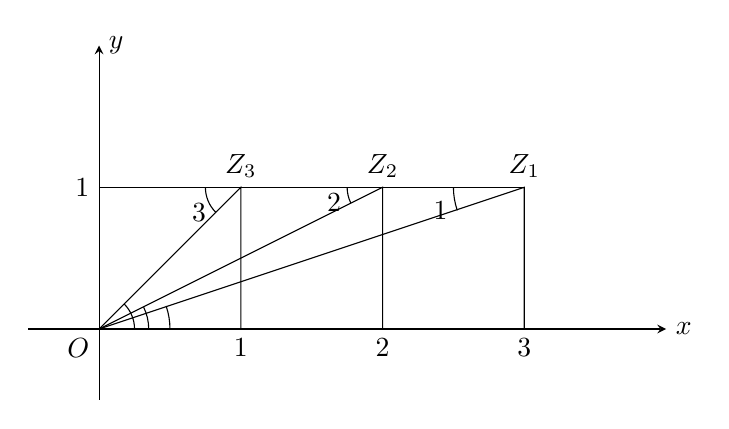
\begin{tikzpicture}[>=stealth, scale=1.8]
\draw[->](-.5,0)--(4,0)node[right]{$x$};    
\draw[->](0,-.5)--(0,2)node[right]{$y$};    
\foreach \x/\y in {1/3,2/2,3/1}
{
    \node at (\x,0)[below]{$\x$};
    \draw(\x,0)--(\x,1)node[above]{$Z_{\y}$}--(0,0);
}
\draw(0,1)node[left]{1}--(3,1);
\node[below left]{$O$};

\draw(1-.25,1) arc (180:180+45:.25)node[left]{$3$};
\draw(2-.25,1) arc (180:180+26:.25)node[left]{$2$};
\draw(3-.5,1) arc (180:180+19:.5)node[left]{$1$};

\draw(.25,0)arc (0:45:.25);
\draw(.35,0)arc (0:26:.35);
\draw(.5,0)arc (0:19:.5);


\end{tikzpicture}
    \caption{}
\end{figure}

\begin{solution}
 如图建立坐标系以确定复平面,不在轴上的三个正
方形顶点设为$Z_1,Z_2,Z_3$.显然,它们分别对应着复数$3+i$, $2+i$, $1+i$; 由于平行线的内错角相等,因而$\angle 1$、$\angle 2$、$\angle 3$ 分别等于复数$3+i$, $2+i$,$1+i$的幅角的主值。

又由复数的乘、除法可知,$\angle 1+\angle 2-\angle 3$就是复数$\frac{(3+i)(2+i)}{1+i}$的幅角,而
\[\frac{(3+i)(2+i)}{1+i}=\frac{5+5i}{1+i}=5\]
它的幅角的主值是0,所以$\angle 1+\angle 2-\angle 3=0$.
\end{solution}

\begin{ex}
\begin{enumerate}
    \item 计算
\begin{enumerate}[(1)]
    \item $\sqrt{2}\left(\pc{\frac{\pi}{6}}\right)\cdot \frac{\sqrt{2}}{2}\left(\pc{\frac{\pi}{4}}\right)$
    \item $2\left(\pc{\frac{4\pi}{3}}\right)\cdot 3\left(\pc{\frac{5\pi}{6}}\right)$
    \item $\sqrt{3}(\pc{240^{\circ}})\cdot \frac{\sqrt{3}}{3}(\pc{150^{\circ}})$
    \item $4(\pc{18^{\circ}})\cdot [\pcx{-306^{\circ}}]\cdot 5(\pc{108^{\circ}})$
\end{enumerate}
\item 用棣美佛定理计算:
\begin{enumerate}[(1)]
    \item $\left[2\sqrt{2}(\pc{18^{\circ}})\right]^5$
    \item $(-1-i)^6$
    \item $\left[\sqrt{3}\left(\pc{\frac{3\pi}{4}}\right)\right]^4$
    \item $(2-i)\cdot \left(-\frac{1}{2}+\frac{\sqrt{3}}{2}i\right)^7$
\end{enumerate}
\item 计算:
\begin{enumerate}[(1)]
    \item $12\left(\pc{\frac{7\pi}{4}}\right)\div 6\left(\pc{\frac{2\pi}{3}}\right)$
    \item $2\div (\pc{45^{\circ}})$
    \item $-i\div 2\left(\pc{\frac{4\pi}{3}}\right)$
    \item $(-i+i)\cdot \sqrt{2}(\pc{120^{\circ}})\div 3(\pc{55^{\circ}})$
\end{enumerate}

\item 你能说明复数除法的几何意义吗?
\item 利用复数证明:在${\rm Rt}\triangle ABC$中,
$\angle C=90^{\circ}$, $AC=3BC$,$E$为$AC$上一点,且$CE=2EA$,则:
\[\angle CBE+\angle CBA-\frac{\pi}{4}=\frac{\pi}{2}\]
\end{enumerate}
\end{ex}

\subsection{复数的开方运算}
开方是乘方的逆运算,求一个复数$a+bi$的$n$次方根,就是求一个数$z$,使得$z^n=a+bi$. 凡满足这一等式的数$z$,就叫做复数$a+bi$的$n$次方根.

设$a+bi=r(\cos\theta+i\sin\theta)$, $z=\rho(\cos\varphi+i\sin\varphi)$,
则对于任意自然数$n$,都有
\[r(\cos\theta+i\sin\theta)=[\rho(\cos\varphi+i\sin\varphi)]^n=\rho^n(\cos n\varphi+i\sin n\varphi)\]

由于两复数相等,它们的模相等,而它们的幅角可以相差$2\pi$的整数倍,所以
\[\begin{cases}
    \rho^n=r\\
    n\varphi=\theta+2k\pi\quad (k\in\Z)
\end{cases}\]

因而可得
\[\rho=\sqrt[n]{r},\qquad \varphi=\frac{\theta+2k\pi}{n}\]

因此,复数$r(\pc{\theta})$的$n$次方根是
\[\sqrt[n]{r}\left(\pc{\frac{2k\pi+\theta}{n}}\right)\]
其中,当$k=0,1,\ldots,n-1$各值时,可以得到上式的$n$个不同值;当$k$继续取$n,n+1,\ldots$以及其它的值时,由于正弦、余弦函数都是以$2\pi$为周期,上式的值又重复出现$k$取$0,1,\ldots,n-1$时的同样结果.所以,复数的$n$次($n\in\N$)方根是$n$个复数,它们的模都等于这个复数的模的$n$次算术根,它们的幅角分别等于这个复数的幅角与$2\pi$的$0,1,\ldots,n-1$倍的和的$n$分之一. 即
\[\sqrt[n]{r(\pc{\theta})}=\sqrt[n]{r}\left(\pc{\frac{\theta+2k\pi}{n}}\right)\quad (k=0,1,\ldots,n-1)\]

\begin{rmk}
在复数范围内,$\sqrt[n]{z}$应表示$n$个复数,这$n$个复数都是$z$的$n$次方根,为了区别于在实数范围内,$\sqrt[n]{z}$仅表示算术根,我们约定:被开方数是实数时,$\sqrt[n]{z}\; (a\in\R)$仍表示算术根(单值),$\sqrt[n]{a+0i}$或$\sqrt[n]{a(\pc{0})}\; (a>0)$或$\sqrt[n]{|a|(\pc{\pi})}$都表示$n$个$n$次方根(多值). 至于被开方数是虚数时,$\sqrt[n]{a+bi}\; (b\ne 0)$或$\sqrt[n]{r(\pc{\theta})}$都表示$n$个方根.
\end{rmk}

\begin{example}
    求$i$的平方根.
\end{example}

\begin{solution}
$\because\quad i=\pc{\frac{\pi}{2}}$

$\therefore\quad \sqrt{i}=\pc{\frac{\frac{\pi}{2}+2k\pi}{2}}=\pcx{\frac{\pi}{4}+k\pi}\quad (k=0,1)$

因此,$i$的平方根是
\[\begin{split}
z_1=\pc{\frac{\pi}{4}}=\frac{\sqrt{2}}{2}+\frac{\sqrt{2}}{2}i\qquad &\text{($k=0$时)}\\
z_2=\pc{\frac{5\pi}{4}}=-\frac{\sqrt{2}}{2}-\frac{\sqrt{2}}{2}i\qquad &\text{($k=1$时)}
\end{split}\]
\end{solution}

\begin{example}
    求$-1+i$的四次方根.
\end{example}

\begin{solution}
$\because\quad -1+i=\sqrt{2}\left(\pc{\frac{3\pi}{4}}\right)$

$\therefore\quad \sqrt[4]{-1+i}=\sqrt[8]{2}\left(\pc{\frac{\frac{3\pi}{4}+2k\pi}{4}}\right)\quad (k=0,1,2,3)$

因此,$-1+i$的四次方根是:
\[\begin{split}
z_1=\sqrt[8]{2}\left(\pc{\frac{3\pi}{16}}\right)\qquad & (k=0)\\
z_2=\sqrt[8]{2}\left(\pc{\frac{11\pi}{16}}\right)\qquad & (k=1)\\
z_3=\sqrt[8]{2}\left(\pc{\frac{19\pi}{16}}\right)\qquad & (k=2)\\
z_4=\sqrt[8]{2}\left(\pc{\frac{27\pi}{16}}\right)\qquad & (k=3)\\
\end{split}\]
\end{solution}

\begin{example}
    求$-3$的平方根.
\end{example}

\begin{solution}
$\because\quad -3=3(\pc{\pi})$

$\therefore\quad \sqrt{-3+0i}=\sqrt{3}\left(\pc{\frac{\pi+2k\pi}{2}}\right)\quad (k=0,1)$

因此,$-3$的平方根有两个复数:
\[\begin{split}
z_1&=\sqrt{3}\left(\pc{\frac{\pi}{2}}\right)=\sqrt{3}i\\
z_2&=\sqrt{3}\left(\pc{\frac{3\pi}{2}}\right)=-\sqrt{3}i\\
\end{split}\]
\end{solution}

一般来说,在复数范围内,任一个负实数$-a$有两个平方根:$\pm\sqrt{a}i$.

这样一来,以前在解实系数一元二次方程$ax^2+bx+c=0$时,如果$b^2-4ac<0$,在实数范围内无解. 现在,在复数范围内,方程就有两个解:
\[x=\frac{-b\pm\sqrt{-(b^2-4ac)}i}{2a}\qquad (b^2-4ac<0)\]
显然,这两个解是一对共轭复数.

\begin{example}
    解方程$x^2-2x+6=0$.
\end{example}

\begin{solution}
$\because\quad \Delta=b^2-4ac=4-24=-20<0$

$\therefore\quad x=\frac{2\pm\sqrt{20}i}{2}=1\pm\sqrt{5}i$
\end{solution}

由以上可知,复数集$\mathbb{C}$对于开方运算是封闭的,这是复数系不同于实数系的一个重要性质.

利用复数开方的方法,我们可以解一些特殊的高次方程,例如,

形如$a_nx^n+a_0=0\; (a_n\ne 0)$的方程,我们叫做二项方程,就可以完整地解出,即,首先化成$x^n=b\quad \left(b=-\frac{a_0}{a_n}\right)$的形式,从而解出$x$的$n$个值.

\begin{example}
    解方程$x^5+243=0$.
\end{example}

\begin{solution}
$\because\quad x^5=-243=243(-1+0i)=243(\pc{\pi})$

$\therefore\quad x=\sqrt[5]{243}\left(\pc{\frac{\pi+2k\pi}{5}}\right)\quad (k=0,1,2,3,4)$

即
\[\begin{split}
x_1&=3\left(\pc{\frac{\pi}{5}}\right)\qquad\quad (k=0)\\
x_2&=3\left(\pc{\frac{3\pi}{5}}\right)\qquad (k=1)\\
x_3&=3\left(\pc{\pi}\right)\qquad\qquad (k=2)\\
x_4&=3\left(\pc{\frac{7\pi}{5}}\right)\qquad (k=3)\\
x_5&=3\left(\pc{\frac{9\pi}{5}}\right)\qquad (k=4)\\
\end{split}\]
\end{solution}

仔细观察这五个解可以发现:它们的模都相同,它们的幅角依次相差$\frac{2\pi}{5}$:因此,这个方程的五个解所对应的复平面内的五个点是均匀地分布在以原点为圆心,以3为半径的圆周上(图1.11).这就是此方程的解的几何意义。
\begin{figure}[htp]
    \centering
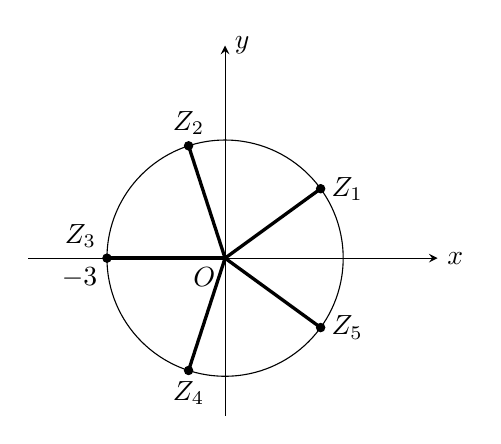
\begin{tikzpicture}[>=stealth]
\draw[->](-2.5,0)--(2.7,0)node[right]{$x$};
\draw[->](0,-2)--(0,2.7)node[right]{$y$};
\draw(0,0)node[below left]{$O$} circle(1.5);
\coordinate (Z1) at (36:1.5);
\coordinate (Z2) at (36*3:1.5);
\coordinate (Z3) at (36*5:1.5);
\coordinate (Z4) at (36*7:1.5);
\coordinate (Z5) at (36*9:1.5);
\draw[very thick](0,0)--(Z1)node[right]{$Z_1$};
\draw[very thick](0,0)--(Z2)node[above]{$Z_2$};
\draw[very thick](0,0)--(Z3)node[above left]{$Z_3$};
\draw[very thick](0,0)--(Z4)node[below]{$Z_4$};
\draw[very thick](0,0)--(Z5)node[right]{$Z_5$};
\node at (-1.5,0)[below left]{$-3$};
\foreach \x in {1,2,3,4,5}
{
    \draw[fill](Z\x) circle(1.5pt);
}


\end{tikzpicture}
    \caption{}
\end{figure}

一般地,二项方程$x^n=b\; (b\in\mathbb{C})$有$n$个复数根,这些根的几何意义是复平面内的$n$个点(或向量),这些点(或向量的终点)均匀地分布在以原点为圆心,以$\sqrt[n]{|b|}$为半径的圆上.

还要进一步指出:对一般的实系数$n$次方程在复数集内也是恰有$n$个根,但未必都是实数根,可能会有虚根(如例1.25).

可以证明,实系数方程的虚根总是成对地出现的,即

\begin{blk}{定理4(虚根成对定理)}
如果$z=a+bi$是实系数方程
$f(x)=a_nx^n+a_{n-1}x^{n-1}+\cdots+a_1x+a_0=0$
的一个根,那么$z=a-bi$也是方程$f(x)=0$的一个根.
\end{blk}

\begin{proof}
    由于$z=a+bi$是方程的根,所以
\[f(z)=f(a+bi)=0\]
但根据习题1 2第15题(2)已证明的结论,应有
\[f(\bar z)=f(a-bi)=f(\overline{a+bi})=\bar 0=0\]
因此,$\bar z=a-bi$也是方程$f(x)=0$的根.
\end{proof}

\begin{example}
    已知方程
$2x^4-x^3+5x^2+13x+5=0$
的一个根为1,求这个方程的其余根.
\end{example}

\begin{solution}
    这是一个实系数一元四次方程,由定理4及已知一根$1-2i$可知,这一方程必有根$1+2i$.

又由因式定理知:$(x-1+2i)(x-1-2i)=x^2-2x+5$是方程左边的因式,利用长除法可得
\[2x^4-x^3+5x^2+13x+5=(2x^2+3x+1)(x^2-2x+5)\]

所以只要解方程$2x^2+3x+1=0$的根:$x_1=-1$, $x_2=-\frac{1}{2}$,就可知:

原方程的其余三根为$1+2i,\; -1,\; -\frac{1}{2}$.
\end{solution}

\begin{ex}
\begin{enumerate}
    \item 直接说出以下各数的平方根:
\[-4,\quad -2.25,\quad -3,\quad -t\; (t\in\R^+),\quad -m^2\; (m\in\R)\]
\[a\; (a\in\R),\quad a-b\; (a,b\in\R)\]
    \item 求下列各数的方根:
\begin{enumerate}[(1)]
    \item $-i,\; \sqrt{2}-\sqrt{2}i,\; -\frac{1}{2}+\frac{\sqrt{3}}{2}i$的平方根;
    \item $27,\; 1+i$的立方根;
    \item $-i$的五次方根.
\end{enumerate}
    \item 解方程(在复数范围内):
\begin{multicols}{2}
\begin{enumerate}[(1)]
    \item $x^2+x+16=0$
    \item $x^3-1=0$
    \item $x^4+16=0$
    \item $x^5-i=0$
\end{enumerate}
\end{multicols}
    \item 已知方程$4x^4-2x^3-x-1=0$有一个根为$-\frac{i}{\sqrt{2}}$,试求这个方程的其余三个根.
\end{enumerate}
\end{ex}


\subsection{单位根}
我们把方程$x^n=1$在复数范围内的$n$个根,叫做$n$次单位根.也就是在复数范围内,1的$n$个不同的$n$次方根,都叫$n$次单位根. 即

$\because\quad x^n=1=\pc{0}$

$\therefore\quad x=1\cdot \left(\pc{\frac{2k\pi}{n}}\right)\quad (k=0,1,\ldots,n-1)$

这样可得出$n$个单位根:
\[\begin{split}
x_1&=\pc{0}=1\qquad \qquad \text{(当$k=0$时)}\\
x_2&=\pc{\frac{2\pi}{n}}\qquad \qquad \text{(当$k=1$时)}\\
x_3&=\pc{\frac{4\pi}{n}}\qquad \qquad \text{(当$k=2$时)}\\
\cdots&\cdots\cdots\\ 
x_n&=\pc{\frac{2(n-1)\pi}{n}}\qquad \text{(当$k=n-1$时)}\\
\end{split}\]

由二项方程解的几何意义可以知道:$n$个不同的单位根可用复平面内以原点为圆心的单位圆的一个内接正$n$边形顶点来表示.

\begin{example}
    求三次单位根.
\end{example}

\begin{solution}
$\because\quad x^3=1=\pc{0}$

$\therefore\quad x=\pc{\frac{2k\pi}{3}}\quad (k=0,1,2)$

因此,三个三次单位根为(如图1.12):
\[\begin{split}
    x_1&=\pc{0}=1\\
    x_2&=\pc{\frac{2\pi}{3}}=-\frac{1}{2}+\frac{\sqrt{3}}{2}i\\
    x_3&=\pc{\frac{4\pi}{3}}=-\frac{1}{2}-\frac{\sqrt{3}}{2}i\\
\end{split}\]
\end{solution}

\begin{minipage}{.45\textwidth}
\centering
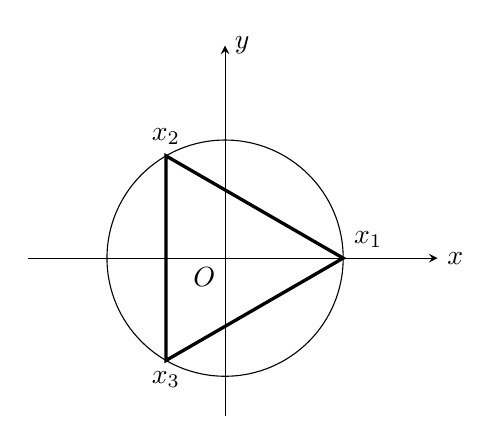
\begin{tikzpicture}[>=stealth]
\draw[->](-2.5,0)--(2.7,0)node[right]{$x$};
\draw[->](0,-2)--(0,2.7)node[right]{$y$};
\draw(0,0)node[below left]{$O$} circle(1.5);
\draw[very thick](1.5,0)node[above right]{$x_1$}--(120:1.5)node[above]{$x_2$}--(240:1.5)node[below]{$x_3$}--cycle;

\end{tikzpicture}
\captionof{figure}{ }
\end{minipage}\hfill
\begin{minipage}{.45\textwidth}
\centering
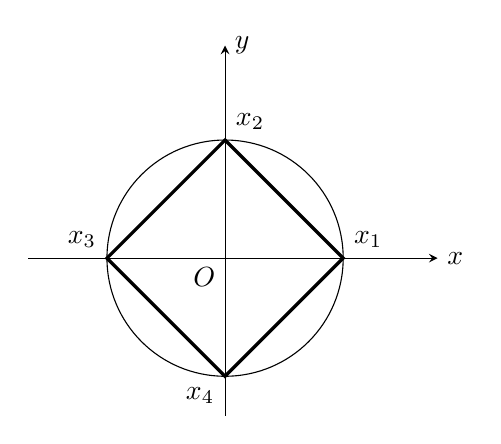
\begin{tikzpicture}[>=stealth]
    \draw[->](-2.5,0)--(2.7,0)node[right]{$x$};
    \draw[->](0,-2)--(0,2.7)node[right]{$y$};
    \draw(0,0)node[below left]{$O$} circle(1.5);
\draw[very thick](1.5,0)node[above right]{$x_1$}--(0,1.5)node[above right]{$x_2$}--(-1.5,0)node[above left]{$x_3$}--(0,-1.5)node[below left]{$x_4$}--cycle;

\end{tikzpicture}
\captionof{figure}{ }
\end{minipage}

\begin{example}
    求四次单位根
\end{example}

\begin{solution}
$\because\quad x^4=1$

$\therefore\quad x=\pc{\frac{2k\pi}{4}}\quad (k=0,1,2,3)$

因此,四个四次单位根为(如图1.13):
\begin{center}
\begin{tabular}{p{.2\textwidth}p{.15\textwidth}p{.2\textwidth}p{.15\textwidth}}
    $x_1=1$& $(k=0)$ & $x_2=i$ & $(k=1)$\\
    $x_3=-1$ &$ (k=2)$& $x_4=-i$ & $(k=3)$\\
\end{tabular} 
\end{center}
\end{solution}


如果用复数的向量表示法
来看这$n$个不同的$n$次单位根的话,我们会发现单位根之间还有一定的关系.

\begin{figure}[htp]
    \centering
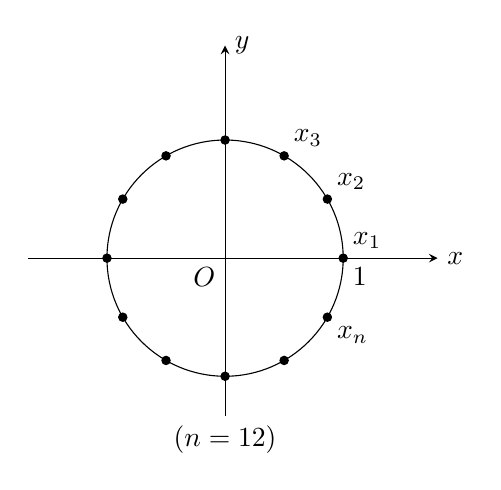
\begin{tikzpicture}[>=stealth]
    \draw[->](-2.5,0)--(2.7,0)node[right]{$x$};
    \draw[->](0,-2)node[below]{$(n=12)$}--(0,2.7)node[right]{$y$};
    \draw(0,0)node[below left]{$O$} circle(1.5);
\foreach \x in {0,1,2,...,11}
{
    \draw[fill](\x*30:1.5) circle(1.5pt);
}
\node at (1.5,0)[below right]{1};
\node at (0:1.5)[above right]{$x_1$};
\node at (30:1.5)[above right]{$x_2$};
\node at (60:1.5)[above right]{$x_3$};
\node at (-30:1.5)[below right]{$x_n$};


\end{tikzpicture}
    \caption{}
\end{figure}




\begin{enumerate}
\item 如图1.14所示,在复平面上$n$个$n$次单位根正好将单位圆$n$等分,其中:
$x_1=1$,单位向量$\VEC{Ox_1}$旋转$\frac{2\pi}{n}$
得:$x_2=\pc{\frac{2\pi}{n}}$
记为$\omega$;再旋转$\frac{2\pi}{n}$
得:$x_3=\pc{\frac{4\pi}{n}}=\omega^2$;再旋转$\frac{2\pi}{n}$可一样地
得:$x_4=\pc{\frac{6\pi}{n}}=\omega^3$,……

同理可得:
\[x_n=\pc{\frac{2(n-1)\pi}{n}}=\omega^{n-1}\]

因此,设$\omega=\pc{\frac{2\pi}{n}}$,则$n$个$n$次单位根又可写成:
\[1,\; \omega,\; \omega^2,\; \ldots, \omega^{n-1}\]

\item 进一步考虑这$n$个单位根的关系,可以发现:

\[\begin{split}
    \because\quad \omega^{n-1}=\pc{\frac{2(n-1)\pi}{n}}&=\pcx{\frac{-2\pi}{n}}\\
    &=\cos\frac{2\pi}{n}-i\sin\frac{2\pi}{n}=\overline{\omega}
\end{split}\]

$\therefore\quad \omega^{n-1}=\overline{\omega}=\frac{1}{\omega}=\omega^{-1}$

同理可得:\[\omega^{n-2}=\overline{\omega^2}=\omega^{-2},\ldots\]

\[\begin{cases}
\text{当$n$为偶数时}& \omega^{\tfrac{n}{2}+1}=\overline{\omega^{\tfrac{n}{2}-1}}=\omega^{-\left(\tfrac{n}{2}-1\right)}=\omega^{-\tfrac{n}{2}+1}\\
\text{当$n$为奇数时}& \omega^{\tfrac{n+1}{2}}=\overline{\omega^{\tfrac{n-1}{2}}}=\omega^{-\tfrac{n-1}{2}}
\end{cases}\]
所以,这$n$个$n$次单位根还可以写成:
\begin{itemize}
    \item 当$n$为偶数时(如例1.29):
\[1,\; \omega,\; \omega^2,\;\ldots,\;  \omega^{\tfrac{n}{2}-1},\;-1,\;  \omega^{-\left(\tfrac{n}{2}-1\right)},\; \ldots, \;  \omega^{-2},\; \omega^{-1}\]
或
\[1,\; \omega,\; \omega^2,\;\ldots,\;  \omega^{\tfrac{n}{2}-1},\;-1,\;  \overline{\omega^{\tfrac{n}{2}-1}},\; \ldots, \;  \overline{\omega^{2}},\; \overline{\omega}\]

\item 当$n$为奇数时(如例1.28):
\[1,\; \omega,\; \omega^2,\;\ldots,\;  \omega^{\tfrac{n-1}{2}},\;  \omega^{-\tfrac{n-1}{2}},\; \ldots, \;  \omega^{-2},\; \omega^{-1}\]
或
\[1,\; \omega,\; \omega^2,\;\ldots,\;  \omega^{\tfrac{n-1}{2}},\;  \overline{\omega^{\tfrac{n-1}{2}}},\; \ldots, \;  \overline{\omega^{2}},\; \overline{\omega}\]
其中,$\omega=\pc{\frac{2\pi}{n}}$.
\end{itemize}

例如,三次单位根为$1,\; \omega,\; \omega^{-1}$(或$\bar\omega$),其中
\[\omega=\pc{\frac{2\pi}{3}}=-\frac{1}{2}+\frac{\sqrt{3}}{2}i\]

又如,四次单位根为$1,\; \omega,\; -1,\; \omega^{-1}$(或$\bar\omega$),其中
\[\omega=\pc{\frac{2\pi}{4}}=i\]

\item 利用单位根,可以方便地求出任一个正实数$ca>0$且$c\ne 1$的$n$个$n$次方根.

这就是:若$a>0$且$a\ne 1$,则$a$的$n$个$n$次方根即方程$x^n=a$的解为:
\[\begin{cases}
x_1=\sqrt[n]{a}\\
x_2=\sqrt[n]{a}\cdot \omega\\
x_3=\sqrt[n]{a}\cdot \omega^2\\
\cdots\cdots\cdots\\
x_n=\sqrt[n]{a}\cdot \omega^{n-1}\\
\end{cases}\qquad \text{这里$\omega=\pc{\frac{2\pi}{n}}$是单位根之一}\]
\end{enumerate}

\begin{ex}
试求出六次和七次单位根,并分别检验它们之间的关系.
\end{ex}

\section*{习题1.3}
\begin{enumerate}
    \item 把下列复数化成三角形式表示:
\begin{multicols}{3}
\begin{enumerate}[(1)]
    \item 6
    \item $6i$
    \item $1+i$
    \item $\frac{1}{2}-\frac{\sqrt{3}}{2}i$
    \item $-\sqrt{2}-\sqrt{2}i$
\end{enumerate}
\end{multicols}

\item 把下列复数化为代数形式表示,并画出复平面上相应的向量来:
\begin{multicols}{2}
\begin{enumerate}[(1)]
    \item $3\sqrt{2}\left(\pc{\frac{\pi}{4}}\right)$
    \item $2\left(\pc{\frac{11\pi}{6}}\right)$
    \item $\pc{\pi}$
    \item $\sqrt{3}\left[\pcx{-\frac{2\pi}{3}}\right]$
    \item $\pcx{k\cdot \frac{\pi}{4}}$
    
    $(k=0,1,2,\ldots,6,7)$
\end{enumerate}
\end{multicols}

\item 计算
\begin{enumerate}[(1)]
    \item $\sqrt{3}\left(\pc{\frac{\pi}{3}}\right)\cdot 2\sqrt{3}\left(\pc{\frac{\pi}{6}}\right)$
    \item $\sqrt{10}\left(\pc{\frac{\pi}{2}}\right)\cdot \sqrt{2}\left(\pc{\frac{\pi}{4}}\right)$
\end{enumerate}

\item 下列复数是不是三角形式?如果不是,请化成三角形式表示:
\begin{multicols}{2}
\begin{enumerate}[(1)]
    \item $\cos\frac{\pi}{6}-i\sin\frac{\pi}{6}$
    \item $\sqrt{2}\left(\cos\frac{4\pi}{3}+i\sin\frac{2\pi}{3}\right)$
    \item $7\left(\sin\frac{3\pi}{4}+i\cos\frac{3\pi}{4}\right)$
    \item $3\left(\cos\frac{5\pi}{6}+i\sin\frac{-7\pi}{6}\right)$
\end{enumerate}
\end{multicols}

\item 求证:
\begin{enumerate}[(1)]
    \item $\sqrt{2}(\pc{75^{\circ}})\cdot \sqrt{2}\left(\pc{15^{\circ}}\right)=2i$
    \item $(\cos3\theta-i\sin3\theta)(\cos2\theta-i\sin2\theta)=\cos5\theta-i\sin5\theta$
\end{enumerate}

\item 如图1.15所示,菱形$OABC$的一个内角$\angle AOC=\frac{\pi}{4}$,且$A$点所对应的复数为$2+i$, 试求,$B$、$C$两点各对应的复数.

\begin{figure}[htp]
    \centering
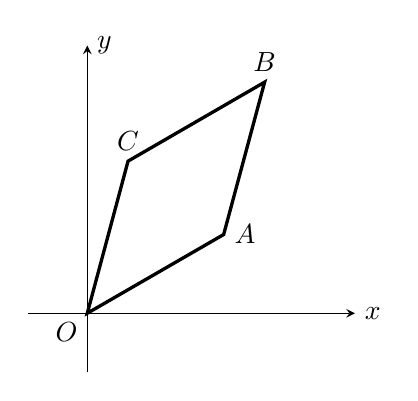
\begin{tikzpicture}[>=stealth]
    \draw[->](-.75,0)--(3.4,0)node[right]{$x$};
    \draw[->](0,-.75)--(0,3.4)node[right]{$y$};
    \node[below left]{$O$} ;
    \coordinate (A) at (30:2);
    \coordinate (C) at (75:2);
    \coordinate (B) at (105/2:3.7);
    \draw[very thick](0,0)--(A)node[right]{$A$}--(B)node[above]{$B$}--(C)node[above]{$C$}--cycle;
\end{tikzpicture}
    \caption{}
\end{figure}


\item 已知下列各复数$z$,求$\left|\frac{1}{z}\right|$及$\arg\left(\frac{1}{z}\right)$
\begin{multicols}{2}
\begin{enumerate}[(1)]
    \item $z=2\left(\pc{\frac{\pi}{12}}\right)$
    \item $z=\cos\frac{\pi}{6}-i\sin\frac{\pi}{6}$
    \item $z=\frac{1-i}{\sqrt{2}}$
\end{enumerate}    
\end{multicols}

\item 把复数$3-\sqrt{3}i$对应的向量旋转$\frac{\pi}{3}$,所得向量相对应的复数是什么?

\item 用棣美佛定理计算:
\begin{multicols}{2}
\begin{enumerate}[(1)]
    \item $[2(\pc{15^{\circ}})]^6$
    \item $\left[\frac{1}{\sqrt{2}}(\pc{225^{\circ}})\right]^4$
    \item $(1+\sqrt{3}i)^4$
    \item $(2-2\sqrt{3}i)^4$
    \item $\frac{(\sqrt{3}+i)^5}{-1+\sqrt{3}i}$
    \item $\left(\frac{2+2i}{1-\sqrt{3}i}\right)^8$
\end{enumerate}
\end{multicols}

\item 用棣美佛定理证明:
\begin{enumerate}[(1)]
    \item $\cos2\theta=\cos^2\theta-\sin^2\theta,\qquad \sin2\theta=2\sin\theta\cdot \cos\theta$
    \item $\cos3\theta=4\cos^3\theta-3\cos\theta,\qquad \sin3\theta=2\sin^2\theta-4\sin\theta$
\end{enumerate}

\item 设$n\in\N$,$n$取何值时,$(1+\sqrt{3})^n$是一个实数?

\item 计算:
\begin{enumerate}[(1)]
    \item $10\left(\pc{\frac{2\pi}{3}}\right)\div 2\left(\pc{\frac{\pi}{6}}\right)$
    \item $-10i\div 6\left(\pc{\frac{\pi}{6}}\right)$
\end{enumerate}

\item 求证:
\begin{enumerate}[(1)]
    \item $\frac{1}{\cos\theta+i\sin\theta}=\cos\theta-i\sin\theta$
    \item $(\pc{\theta})^{-n}=\pcx{-n\theta}\quad (n\in\mathbb{N})$
    \item $(\cos\theta-i\sin\theta)^n=\cos n\theta-i\sin n \theta\quad (n\in\N)$
\end{enumerate}

\item 利用复数证明余弦定理.

\item 化简:
\begin{enumerate}[(1)]
    \item $\frac{(\pc{7\theta})(\pc{2\theta})}{(\pc{5\theta})(\pc{3\theta})}$
    \item $\frac{\cos\varphi-i\sin\varphi}{\pc{\varphi}}$
    \item $\frac{\pc{\alpha}}{\sin\alpha+i\cos\alpha}$
\end{enumerate}
\item 在复数范围内解下列方程:
\begin{multicols}{2}
\begin{enumerate}[(1)]
    \item $4x^2+9=0$
    \item $2(x^2+4)=5x$
    \item $(x-3)(x-5)=-2$
    \item $\frac{1}{x+3}-\frac{1}{x}=1$
    \item $x^4+3x^2+1=0$
    \item $\frac{x}{x^2+1}+\frac{x^2+1}{x}-\frac{5}{2}=0$
\end{enumerate}
\end{multicols}
\item 解下列方程组:
\begin{multicols}{2}
\begin{enumerate}[(1)]
    \item $\begin{cases}
a+b=2\\ab=2        
    \end{cases}$
    \item $\begin{cases}
        x^2+y^2=0\\
        xy=1
    \end{cases}$
\end{enumerate}
\end{multicols}

\item 求:
\begin{enumerate}[(1)]
    \item $8\left(\pc{\frac{\pi}{3}}\right)$的六次方根;
    \item $-2i$的五次方根.
\end{enumerate}
\item 求:六次单位根、七次单位根,并在复平面上用向量表示出来.

\item 解下列方程:
\begin{multicols}{2}
\begin{enumerate}[(1)]
    \item $x^3+1=i$
    \item $x^4+16=0$
    \item $x^{10}-32x^5+1024=0$
    \item $x^{12}+63x^6-64=0$
\end{enumerate}
\end{multicols}

\item 求证:
\begin{enumerate}[(1)]
    \item 不经计算证明$\left|\frac{a+bi}{a-bi}\right|\equiv 1$
    \item 有相同幅角的两个复数之比必为实数;
    \item 复平面上四个点$Z_1$, $Z_2$, $Z_3$, $Z_4$共圆或共直线的充分必要条件是:
\[\left.\frac{Z_3-Z_1}{Z_3-Z_2}\right/\frac{Z_4-Z_1}{Z_4-Z_2} \text{ 为实数}\]
\end{enumerate}
\end{enumerate}

\section{复数的指数形式}
我们已经学习了复数的代数形式、三角形式以及它们的运算.在科学技术,特别是在电工和无线电计算中,常要涉及复数或三角函数的变换和计算,为方便还采用复数的另一种形式——复数的指数形式,在这一节将学习复数的指数形式及其运算、应用.

\subsection{复数的指数形式及其运算}
我们首先引进一个著名的公式——欧拉公式:
\[e^{i\theta}=\pc{\theta}\]
其中$e=2.71828\cdots$是一个重要的常数,也就是自然对数的底数.

欧拉公式在以后的“复变函数论”中可以证明。这个公式表明了:模为1、幅角为$\theta$的复数$\pc{\theta}$与以$e$为底的复指数函数的关系,从这个公式出发,对任一个复数
\[z=a+bi=r(\pc{\theta})\]
就可以表示成$z=r\cdot e^{i\theta}$的形式,我们就把这一表达式叫做复数的指数形式.

例如:
\begin{itemize}
    \item 复数$\pc{\frac{\pi}{2}}$的指数形式为$e^{i\tfrac{\pi}{2}}$
    \item 复数$3\left(\pc{\frac{\pi}{4}}\right)$的指数形式为$3e^{i\tfrac{\pi}{4}}$
\end{itemize}

这样,同一个复数,就有三种不同形式的表达方法——代数形式、三角形式、指数形式.
如:
\[\begin{split}
    \frac{1}{2}+\frac{\sqrt{3}}{2}i&=\pc{\frac{\pi}{3}}=e^{i\tfrac{\pi}{3}}\\
    -2\sqrt{3}+2i&=4\left(\pc{\frac{5\pi}{6}}\right)=4e^{i\tfrac{5\pi}{6}}
\end{split}\]

复数的指数形式便利于乘、除、乘方及开方运算.因为可以证明原有在实数范围内的指数运算律它都仍然满足. 这就是:

设$z_1=r_1e^{i\theta_1}$,$z_2=r_2e^{i\theta_2}$,则有
\[\begin{split}
    z_1\cdot z_2&=\left(r_1e^{i\theta_1}\right)\cdot \left(r_2e^{i\theta_2}\right)\\
    &=r_1(\pc{\theta_1})\cdot r_2(\pc{\theta_2})\\
    &=r_1r_2[\pcx{\theta_1+\theta_2}]=r_1r_2\cdot e^{i(\theta_1+\theta_2)}
\end{split}\]
即
\[r_1e^{i\theta_1}\cdot r_2e^{i\theta_2}=r_1r_2 e^{i(\theta_1+\theta_2)}\]

同理可证:
\[\begin{split}
    \frac{z_1}{z_2}&=\frac{r_1e^{i\theta_1}}{r_2e^{i\theta_2}}=\frac{r_1}{r_2}\cdot e^{i(\theta_1-\theta_2)}\quad (z_2\ne 0)\\
z^n_1&=(r_1e^{i\theta_1})^n=r^n_1 \cdot e^{i n\theta_1}\quad (n\in\N)
\end{split} \]
$z_1$的$n$次方根:$\sqrt[n]{z_1}=\sqrt[n]{r_1e^{i\theta_1}}=\sqrt[n]{r_1}e^{i\tfrac{\theta_1+2k\pi}{n}}\quad (k=0,1,\ldots,n-1)$

\begin{example}
把复数$z=2i$化成指数形式.
\end{example}

\begin{solution}
$\because\quad z=2i=2\left(\pc{\frac{\pi}{2}}\right)$

$\therefore\quad z=2\cdot e^{i\tfrac{\pi}{2}}$
\end{solution}

\begin{example}
已知$z_1=\sqrt{2}\cdot e^{i\left(-\tfrac{\pi}{4}\right)}$,$z_2=\sqrt{5}\cdot e^{i\tfrac{2\pi}{3}}$. 试求:
\begin{multicols}{2}
\begin{enumerate}[(1)]
    \item $z_1\cdot z_2$
    \item $z_1$的平方根
\end{enumerate}
\end{multicols}
要把结果表示成复数的三角形式.
\end{example}

\begin{solution}
\begin{enumerate}[(1)]
    \item \[\begin{split}
z_1\cdot z_2&=\left(\sqrt{2} e^{i\left(-\tfrac{\pi}{4}\right)}\right)\cdot \left(\sqrt{5} e^{i\tfrac{2\pi}{3}}\right)\\
&=\sqrt{10}e^{i\tfrac{5\pi}{12}}=\sqrt{10}\left(\pc{\frac{5\pi}{12}}\right)
    \end{split}\]
\item $\sqrt{\sqrt{2}\cdot e^{i\left(-\tfrac{\pi}{4}\right)}}=\sqrt[4]{2}\cdot e^{i\tfrac{-\tfrac{\pi}{4}+2k\pi}{2}}\quad (k=0,1)$

$\therefore\quad z_1$的两个平方根为
\[\begin{split}
x_1&=\sqrt[4]{2}\cdot e^{i\left(-\tfrac{\pi}{8}\right)}=\sqrt[4]{2}\left(\pc{\frac{15\pi}{8}}\right)\\
x_2&=\sqrt[4]{2}\cdot e^{i\tfrac{7\pi}{8}}=\sqrt[4]{2}\left(\pc{\frac{7\pi}{8}}\right)
\end{split}\]
\end{enumerate}
\end{solution}



\begin{example}
试用$e^{i\theta}$与$e^{-i\theta}$表示$\cos\theta$与$\sin\theta$.    
\end{example}

\begin{solution}
由于
\begin{align}
e^{i\theta}&= \pc{\theta} \tag{1}\\
e^{-i\theta}&= \pcx{-\theta}=\cos\theta-i\sin\theta \tag{2}
\end{align}
(1)(2)联立,可解出
\[\begin{split}
    \cos\theta&=\frac{1}{2}\left(e^{i\theta}+e^{-i\theta}\right)\\
    \sin\theta&=\frac{1}{2}i\left(e^{i\theta}-e^{-i\theta}\right)\\
\end{split}\]
\end{solution}

\begin{ex}
\begin{enumerate}
    \item 将复数$-1$,$2+2i$,$\pc{15^{\circ}}$,$4i$分别表示成指数形式.
    \item 将复数$e^{-i\tfrac{\pi}{2}}$,$3e^{2i}$,$\sqrt{2}e^{i\tfrac{3\pi}{2}}$分别化为三角形式和代数形式.
    \item 用指数形式计算:
\begin{enumerate}[(1)]
    \item $8\left(\pc{\frac{7\pi}{6}}\right)\cdot 2\left(\pc{\frac{\pi}{4}}\right)$
    \item $2\div e^{i\tfrac{\pi}{4}}$
    \item $(1+\sqrt{3}i)^{10}$
    \item 求81的四次方根
\end{enumerate}
\end{enumerate}
\end{ex}

\subsection{证明三角恒等式}

在我们学习过的三角公式和三角恒等式当中,除了公式$\sin(\alpha+\beta)$与$\cos(\alpha+\beta)$是证明棣美佛定理的依据外,其余公式都可以应用复数的指数形式来加以证明.其要点是:首先将公式中的正切、余切、正割、余割诸函数都化为正弦、余弦函数表达;其次再用由复数的指数形式而导出来的公式:(例1.32)
\[\begin{split}
\sin\theta&=\frac{1}{2}i\left(e^{i\theta}-e^{-i\theta}\right)\\
    \cos\theta&=\frac{1}{2}\left(e^{i\theta}+e^{-i\theta}\right)\\
    \end{split}\]
将三角函数转化为指数形式的代数运算;从而达到证明的目的.

\begin{example}
求证:$-2\sin\alpha\cdot \sin\beta=\cos(\alpha+\beta)-\cos(\alpha-\beta)$    
\end{example}

\begin{proof}
$\because\quad \sin\alpha=\frac{1}{2i}\left(e^{i\alpha}-e^{-i\alpha}\right),\quad \sin\beta=\frac{1}{2i}\left(e^{i\beta}-e^{-i\beta}\right)$

\[\begin{split}
\therefore\quad \text{左}&=-2\cdot \frac{1}{4i^2}\left[e^{i(\alpha+\beta)}+e^{-i(\alpha+\beta)}-e^{i(\alpha-\beta)}-e^{i(\beta-\alpha)}\right]\\
&=\frac{1}{2}\left[e^{i(\alpha+\beta)}+e^{-i(\alpha+\beta)}\right]-\frac{1}{2}\left[e^{i(\alpha-\beta)}+e^{-i(\alpha-\beta)}\right]\\
&=\cos(\alpha+\beta)-\cos(\alpha-\beta)=\text{右}
\end{split}\]

$\therefore\quad $原等式成立.
\end{proof}

\begin{example}
求证:$\sin(\alpha+\beta)\cdot \cos(\alpha-\beta)=\sin\alpha\cdot \cos\alpha+\sin\beta\cdot \cos\beta$
\end{example}

\begin{proof}
\[\begin{split}
\text{左式}&=\frac{1}{2i}\left[e^{i(\alpha+\beta)}-e^{-i(\alpha+\beta)}\right]\cdot \frac{1}{2}\left[e^{i(\alpha-\beta)}+e^{-i(\alpha-\beta)}\right]\\
&=\frac{1}{4i}\left[e^{2\alpha i}+e^{2\beta i}-e^{-2\beta i}-e^{-2\alpha i}\right]
\end{split}\]
\[\begin{split}
    \text{右式}&=\frac{1}{2i}\left(e^{i\alpha}-e^{-i\alpha}\right)\cdot\frac{1}{2}\left(e^{i\alpha}+e^{-i\alpha}\right)+\frac{1}{2i}\left(e^{i\beta}-e^{-i\beta}\right)\cdot \frac{1}{2}\left(e^{i\beta}+e^{-i\beta}\right)\\
    &=\frac{1}{4i}\left[e^{2\alpha i}-e^{-2\alpha i}+e^{2\beta i}-e^{-2\beta i}\right]
\end{split}\]

$\because\quad $左式$=$右式

$\therefore\quad $原等式成立.
\end{proof}

对于具有条件$\alpha+\beta+\gamma=\pi$的三角恒等式,应用复数的指数形式加以证明更为有利.

\begin{example}
在$\triangle ABC$中,求证:
\[1+\cos 2A+\cos 2B+\cos 2C+4\cos A\cdot \cos B\cdot \cos C=0\]
\end{example}

\begin{proof}
\[\begin{split}
 \because\quad    4\cos A\cdot \cos B\cdot \cos C &=4\cdot\frac{e^{iA}+e^{-iA}}{2}\cdot\frac{e^{iB}+e^{-iB}}{2}\cdot\frac{e^{iC}+e^{-iC}}{2}\\
 &=\frac{1}{2}\left[e^{i(A+B+C)}+e^{i(B+C-A)}+e^{i(A+C-B)}\right.\\
 &\qquad   +e^{i(A+B-C)}+e^{-i(B+C-A)}+e^{-i(A+C-B)}\\
&\qquad  \left.+e^{-i(A+B-C)}+e^{-i(A+B+C)}\right]\qquad  \qquad  (*)
\end{split}\]

但由于$A+B+C=\pi$,进而有$B+C-A=\pi-2A$, 
$A+C-B=\pi-2B$, $A+B-C=\pi-2C$; 因此可得:
\[\begin{split}
    e^{i(A+B-C)}&=e^{i\pi}=-1\\
    e^{i(B+C-A)}&=e^{i(\pi-2A)}=e^{i\pi}\cdot e^{-2Ai}=-e^{-2Ai}\\
\end{split}\]
同理:$e^{i(A+C-B)}=-e^{-2Bi},\qquad e^{i(A+B-C)}=-e^{-2Ci}$
\[\begin{split}
    e^{-i(A+B+C)}=e^{-i\pi}=-1,\qquad 
    e^{-i(B+C-A)}=-e^{2Ai}\\
    e^{-i(A+C-B)}=-e^{2Bi},\qquad 
    e^{-i(A+B-C)}=-e^{2Ci}
\end{split}\]

将以上结果代入(*)式,得
\[\begin{split}
    4\cos A\cdot \cos B\cdot \cos C &=\frac{1}{2}\left[-2-e^{2Ai}-e^{2Ai}-e^{2Bi}-e^{2Bi}-e^{2Ci}-e^{2Ci}\right]\\
    &=-1-\cos2A-\cos2B-\cos2C
\end{split}\]

$\therefore\quad 1+\cos 2A+\cos 2B+\cos 2C+4\cos A  \cos B  \cos C=0$
\end{proof}

\begin{ex}
利用复数的指数形式,证明以下等式:
\begin{enumerate}
    \item $\sin2\alpha=2\sin\alpha\cdot \cos\alpha$
    \item $\cos^2\beta-\sin^2\alpha=\cos(\alpha+\beta)\cdot \cos(\alpha-\beta)$
\end{enumerate}
\end{ex}

\section*{习题1.4}
\begin{enumerate}
    \item 把下列复数化为指数形式:
\begin{multicols}{3}
\begin{enumerate}[(1)]
    \item $5$
    \item $2+2i$
    \item $-2i$
    \item $1-\sqrt{3}i$
    \item $\pc{\frac{\pi}{4}}$
    \item $\pc{3}$
    \item $1+\pc{\frac{\pi}{3}}$
\end{enumerate}
\end{multicols}
\item 设复数$a+bi=r\cdot e^{i\theta}$,写出复数$a-bi$, $-a+bi$, $-a-bi$的指数形式.
\item 把下列复数化为三角形式及代数形式:
\begin{multicols}{3}
\begin{enumerate}[(1)]
    \item $4e^{i\tfrac{\pi}{6}}$
    \item $\sqrt{3}e^{i\tfrac{2\pi}{3}}$
    \item $e^{-i\tfrac{3\pi}{2}}$
\end{enumerate}
\end{multicols}

\item 试求:复数$e^{i\tfrac{4\pi}{5}}$, $e^{i\tfrac{2\pi}{3}}$ 所对应的向量间的夹角$\alpha\; (0\le \alpha\le \pi)$.
\item 用复数的指数形式计算:
\begin{enumerate}[(1)]
    \item $\sqrt{2}\left(\pc{\frac{4\pi}{3}}\right)\cdot\frac{\sqrt{2}}{4}\left(\pc{\frac{5\pi}{6}}\right)$
    \item $\sqrt{3}(\pc{150^{\circ}})\div \sqrt{2}(\pc{225^{\circ}})$
\end{enumerate}

\item 根据欧拉公式求证:$e^{-i\theta}=(\pc{\theta})^{-1}$.

\item 用复数的指数形式计算:
\begin{multicols}{3}
\begin{enumerate}[(1)]
    \item $(1+\sqrt{3}i)^{10}$
    \item $(\sqrt{3}-i)^8$
    \item $\sqrt[4]{64+0i}$
\end{enumerate}
\end{multicols}

\item 用复数的指数形式证明恒等式:
\begin{enumerate}[(1)]
    \item $\sin\alpha-\sin\beta=2\cos\frac{\alpha+\beta}{2}\cdot \sin\frac{\alpha-\beta}{2}$
    \item $(\sin\alpha+\sin\beta)^2+(\cos\alpha+\cos\beta)^2=4\cos^2\frac{\alpha-\beta}{2}$
\end{enumerate}
\end{enumerate}

\section*{本章内容要点}

一、本章里,我们引进了虚数单位($i^2=-1$),把数的概念扩展到了复数集. 复数的分类如下:
\begin{center}
\begin{tikzpicture}
\node (A) at (0,0)[text width=2cm, align=center]{复数$a+bi$\\$(a,b\in\R)$};
\node (B1) at (2.5,1)[text width=2cm, align=center]{实数\\($b=0$时)}; 
\node (B2) at (2.5,-1)[text width=2cm, align=center]{虚数\\($b\ne 0$时)}; 
\node (C1) at (5,0)[text width=2cm, align=center]{纯虚数\\($a=0$时)}; 
\node (C2) at (5,-2)[text width=2cm, align=center]{非纯虚数\\($a\ne 0$时)}; 
\draw[decorate, decoration={brace, amplitude=5pt}](1.5,-1.3)--(1.5,1.3);
\draw[decorate, decoration={brace, amplitude=5pt}](3.8,-2.3)--(3.8,.3);


\end{tikzpicture}
\end{center}

且复数集$\supset$实数集$\supset$有理数集$\supset$整数集$\supset$自然数集,即:
\[\mathbb{C} \supset \R \supset \mathbb{Q} \supset \Z\supset\N\]

二、复数有四个基本概念:模,幅角,共轭复数,复数的相等;任一个复数有三种表示形式:代数形式$a+bi\; (a,bE\in\R)$,三角形式$r(\pc{\theta})$,其中$r=\sqrt{a^2+b^2}$, $\tan\theta =\frac{b}{a}$,指数形式$re^{i\theta}$;复数$z=a+bi$与复平
面内的点$Z(a,b)$对应,并且和从原点出发的向量$\VEC{OZ}$相对应,因此,复数集$\mathbb{C}$与复平面内的点集,与从原点出发的向量集合之间成一一对应关系,即
\[\mathbb{C}:\; \{a+bi\mid a,b\in\R,\; i^2=-1\} \longleftrightarrow \{Z(a,b)\}\longleftrightarrow \{\VEC{OZ}\}\]

据此,一些平面几何,平面解析几何以及平面向量的问题,也可以通过复数来解决.

三、复数集对于四则运算及乘方,开方运算都是封闭的;复数集保持了数系运算的“通性”,即加法、乘法的交换律、结合律以及乘法对于加法的分配律、数0与1的运算特性等;但复数集不再具有顺序性,对任意两个不全为实数的复数,就不能比较大小.

四、复数的运算法则及其几何意义:
\begin{enumerate}
    \item 加、减法运算用复数的代数形式表达比较方便,即
    \[(a+bi)\pm (c+di)=(a\pm c)+(b\pm d)i\]
    其几何意义是对应的向量相加、减,即“平行四边形”法则和“三角形”法则,特别是两复数的差的模表示复平面内两点间的距离.
    \item 乘、除法,乘方、开方的运算用复数的三角形式或指数形式表达比较方便,即
\[\begin{split}
    r_1(\pc{\theta_1})\cdot r_2(\pc{\theta_2})&=r_1\cdot r_2\left[r_1\pcx{\theta_1+\theta_2}\right]\\
\frac{r_1(\pc{\theta_1})}{r_2(\pc{\theta_2})}&=\frac{r_1}{r_2}\left[r_1\pcx{\theta_1-\theta_2}\right]
\end{split}\]
棣美佛定理:
\[[r(\pc{\theta})]^n=r^n(\pc{n\theta})\]
$n$个$n$次方根:
\[\begin{split}
\sqrt[n]{r(\pc{\theta})}&=\sqrt[n]{r}\left(\pc{\frac{\theta+2k\pi}{n}}\right)\\
&\qquad (k=0,1,2,\ldots,n-1)\quad (n\in\N)    
\end{split} \]
\end{enumerate}

复数的这些运算,都有其几何意义.特别是:复数的相乘对应着平面向量的旋转;$n$个$n$次方根对应着圆内接正$n$边形的顶点,即圆周的$n$等分点,这些结论在应用上很重要.

五、在复数集中,本章学习了在实数集中所不能解的有关问题:
\begin{enumerate}
    \item 当$b^2-4ac<0$时,一元二次方程$ax^2+bx+c=0\; (a\ne 0)$有两个共轭的虚根,即
\[x=\frac{-b\pm i\sqrt{4ac-b^2}}{2a}\]
\item 二项方程$x^n=b\; (b\in\mathbb{C})$有$n$个不同的复数根,即设$x^n=b=r(\pc{\theta})$,则
\[x=\sqrt[n]{r}\left(\pc{\frac{\theta+2k\pi}{n}}\right)\]
当$k=0,1,2,\ldots,n-1$时,可得出$n$个不同的解.

\item 特别地,方程$x^n=1$的复数解,叫做$n$次单位根,若设$\omega=\pc{\frac{2\pi}{n}}$,则当$n$为偶数时,$n$个单位根为
\[1,\; \omega,\; \omega^2,\;\ldots,\;  \omega^{\tfrac{n}{2}-1},\;-1,\;  \overline{\omega^{\tfrac{n}{2}-1}},\; \ldots, \;  \overline{\omega^{2}},\; \overline{\omega}\]
当$n$为奇数时,$n$个单位根为
\[1,\; \omega,\; \omega^2,\;\ldots,\;  \omega^{\tfrac{n-1}{2}},\;  \overline{\omega^{\tfrac{n-1}{2}}},\; \ldots, \;  \overline{\omega^{2}},\; \overline{\omega}\]

\item 实系数一元方程,若有虚根存在,则一定是成对出现,即实系数方程若有根$a+bi\;(b\ne 0)$则必有根$a-bi$.
\end{enumerate}

\section*{复习题一}
\begin{enumerate}
    \item 在复平面上任选一点$Z$(不在原点)表示复数$z$,然后用几何法在平面找出下列各复数的点:
\begin{multicols}{4}
\begin{enumerate}[(1)]
    \item $-z$
    \item $\bar z$
    \item $-\bar z$
    \item $z+\bar z$
    \item $z-\bar z$
    \item $z+|z|$
    \item $z-|z|$
    \item $iz$
    \item $-iz$
    \item $i\bar z$
    \item $-i\bar z$
\end{enumerate}
\end{multicols}

\item 已知$z=a+bi\; (a,b\in\R)$,求下列各复数的实部与虚部:
\begin{multicols}{2}
\begin{enumerate}[(1)]
    \item $z^2$
    \item $z^3$
    \item $\frac{1}{z}$
    \item $v_0 z+\frac{M}{2\pi}\cdot \frac{1}{z}\quad (v_0,M\in\R)$
\end{enumerate}
\end{multicols}

\item 求复数$z=\frac{a^2-b^2+2abi}{ab\sqrt{2}+\sqrt{a^4+b^4}i}$的模.

\item 求证:表示复数$z_0$的点关于直线${\rm Re}(z)={\rm Im}(z)$的对称点表示的是复数$\overline{i z_0}$.

\item 下列方程($t$为实参数)给出了怎样的曲线?
\begin{multicols}{2}
\begin{enumerate}[(1)]
    \item $z=t(1+i)$
    \item $z=a\cos t+ib\sin t$
    \item $z=t+\frac{i}{t}$
    \item $z=t^2+\frac{i}{t}$
\end{enumerate}
\end{multicols}

\item 已知$(x+yi)^3=a+bi$,$a,b,x,y\in\R$,求证:
$\frac{a}{x}+\frac{b}{y}=4(x^2-y^2)$

\item 若$a$,$b$是共轭复数,且$(a+b)-3abi=4-6i$, 试求$a$及$b$.
\item 若$x,y\in\R$, $z=x+y-30-xyi$且$\bar z=60i-|x+yi|$,试求$x$和$y$的值.
\item 若$z=x+yi$,求证:$|z|\le |x|+|y|\le \sqrt{2}|z|$
\item 试判断以下复数,哪些是实数?哪些是纯虚数?($z,z_1,z_2\in\mathbb{C}$)
\begin{multicols}{2}
\begin{enumerate}[(1)]
    \item $z+\bar z$
    \item $z-\bar z$
    \item $z\cdot \bar z$
    \item $z^2-\bar z^2$
    \item $\frac{\left(\frac{1}{z}+\frac{1}{\bar z}\right)(z+\bar z)}{z-\bar z}$
    \item $z_1\cdot \bar z_2-\bar z_1\cdot z_2$
    \item $z_1\cdot \bar z_2+\bar z_1\cdot z_2$
    \item $\frac{z_1\cdot \bar z_2+\bar z_1\cdot z_2}{z_1\cdot \bar z_1-1}$
    \item $\frac{z_1\cdot \bar z_2-\bar z_1\cdot z_2}{i(z_1\cdot \bar z_1+z_2\cdot \bar z_2)}$
    \item $\frac{i(z_1\cdot \bar z_2+z_2\cdot \bar z_1)}{z_1\cdot \bar z_2-\bar z_1\cdot z_2}$
\end{enumerate}
\end{multicols}

\item 设复数$z_1,z_2$分别对应于点$Z_1,Z_2$,求证:
\begin{enumerate}[(1)]
    \item $OZ_1\bot OZ_2$的充要条件是$z_1\cdot \bar z_2+\bar z_1\cdot z_2=0$
    \item $OZ_1$与$OZ_2$共线的充要条件是$z_1\cdot \bar z_2-\bar z_1\cdot z_2=0$
\end{enumerate}

\item 设$\alpha$是复常数,$k$是实常数,$z\in\mathbb{C}$,试说明下述方程在复平面上的图形是什么?
\begin{multicols}{2}
\begin{enumerate}[(1)]
    \item $\alpha\bar z+\bar\alpha\cdot z=k$;
    \item $z\bar z+z\bar\alpha+\alpha\bar z+k=0$.
\end{enumerate}
\end{multicols}
\item 求证:如果$\frac{1}{z}+z\in\R$,那么${\rm Im}(z)=0$或$|z|=1$.
\item 化简:$\left(\frac{1-i}{1+i}\right)^{4\alpha}$,其中$\alpha=\csc10^{\circ}-\sqrt{3}\sec10^{\circ}$.
\item 解方程组
\begin{multicols}{2}
\begin{enumerate}[(1)]
    \item $\begin{cases}
        x+iy=2+4i\\ ix+y=0
    \end{cases}$
    \item $\begin{cases}
        z_1+2z_2=1+i\\  3z_1+iz_2=2-3i
    \end{cases}$
    \item $\begin{cases}
x^2+y^2=6\\        
x^2+y^2=0\\        
x^2+z^2=8i\\        
    \end{cases}$
\end{enumerate}
\end{multicols}

\item 化简
\[\frac{(\cos2\theta-i\sin2\theta)(\pc{\theta})^2}{\pcx{\theta+\varphi}}\cdot \frac{(\pc{2\theta})^2(\cos2\varphi-i\sin2\varphi)}{\pcx{\theta-\varphi}}\]

\item 将下列复数化为三角形式:
\begin{multicols}{2}
\begin{enumerate}[(1)]
    \item $\frac{(\pc{5\varphi})^2}{(\cos3\varphi-i\sin3\varphi)^3}$
    \item $1-\pc{\theta},\quad (0\le\theta\le\pi)$
\end{enumerate}
\end{multicols}

\item 设$x=e^{i\alpha}$, $y=e^{i\beta}$, $z=e^{i\gamma}$,求证:
\[(x+y)(y+z)(z+x)=8xyz\cos\frac{\beta-\gamma}{2}\cdot \cos\frac{\gamma-\alpha}{2}\cdot \cos\frac{\alpha-\beta}{2}\]

\item 设$\sin A+\sin B+\sin C=\cos A+\cos B+\cos C=0$,求证:
\begin{enumerate}[(1)]
    \item $\sin3A+\sin3B+\sin3C=3\sin(A+B+C)$
\item $\cos3A+\cos3B+\cos3C=3\cos(A+B+C)$
\end{enumerate}
\item 在复平面上,$z_1=1$, $z_2=2+i$与$z_3$组成一个正三角形,求$z_3$.
\item 若$z_1,z_2,z_3,z_4$是一个正方形的四个顶点,且$z_1=1+2i$, $z_2=3-5i$, 求$z_3,z_4$.
\item 求证:$\triangle z_1z_2z_3$是等边三角形的充要条件是:
\[z_1^2+z_2^2+z_3^2=z_1\cdot z_2+z_2\cdot z_3+z_3\cdot z_1\]
\item 下列条件表示什么样图形?
\begin{enumerate}[(1)]
    \item ${\rm Im}(z^2)=2$
    \item $|z|=1$且$\arg z\in(0,\pi)$
    \item $0<a\le {\rm Im}(z)\le b$且$\frac{\pi}{4}\le \arg z\le \frac{3\pi}{4}$
\end{enumerate}
\item 你能用复数表示出图中的半圆来吗?(包括边界)

\begin{minipage}{.45\textwidth}
    \centering
\begin{tikzpicture}[>=stealth]
\draw[->](-1.5,0)--(1.5,0)node[right]{$x$};
\draw[->](0,-1)--(0,2)node[right]{$y$};
\draw[pattern=north east lines](1,0)node[below]{2} arc (0:180:1)node[below]{$-2$} --cycle;
\node[below left]{$O$};
\node at (0,1)[above right]{2};    
\end{tikzpicture}
\captionof{figure}{ }
\end{minipage}\hfill
\begin{minipage}{.45\textwidth}
    \centering
\begin{tikzpicture}[>=stealth]
    \draw[->](-1.5,0)--(1.5,0)node[right]{$x$};
\draw[->](0,-1.5)--(0,1.5)node[right]{$y$};
\draw[pattern=north east lines](0,1)node[right]{1} arc (90:180+90:1)node[right]{$-1$}--cycle; 
\node[below right]{$O$};   
\node at (-1,0)[below left]{$-1$};   
\end{tikzpicture}
\captionof{figure}{ }
\end{minipage} 

\item 设$z\in\mathbb{C}$,解方程:
\begin{multicols}{2}
\begin{enumerate}[(1)]
    \item $\frac{1}{2}(z-1)=\frac{\sqrt{3}}{2}(1+z)i$
    \item $(z+1)^8=(1+i)^8$
\end{enumerate}
\end{multicols}

\item 设$z$是虚数,解方程:
\begin{multicols}{2}
\begin{enumerate}[(1)]
    \item $z+|\bar z|=2+i$
    \item $z^2=\bar z$
\end{enumerate}
\end{multicols}

\item 求证:
\begin{enumerate}[(1)]
    \item $|z|=1\; (z\in\mathbb{C})$的充要条件是$z^{-1}=\bar z$;
    \item 共轭虚数的$n\; (n\in\N)$次幂仍是共轭虚数;
    \item 虚数的平方根仍是虚数.
\end{enumerate}

\item 在复数集中解下列方程组:
\begin{enumerate}[(1)]
    \item $\begin{cases}
        x^2+y^2-2xy+3(x+y)-2=0\\
        2(x^2+y^2)-2xy-2(x+y)+15=0
    \end{cases}$
    \item $\begin{cases}
        \frac{x-y}{1+xy}=\frac{1}{3}\\  \frac{x+y}{1-xy}=3
    \end{cases}$
\end{enumerate}    

\item 设三次单位根为$1,\omega,\omega^2$,其中
$\omega=-\frac{1}{2}+\frac{\sqrt{3}}{2}i$,求证:
\begin{enumerate}[(1)]
    \item $1+\omega+\omega^2=0$
    \item $1\cdot \omega\cdot \omega^2=1$
    \item $(1+\omega^2)^4=\omega$
    \item $\begin{vmatrix}
        1&1&\omega\\
        1&1&\omega^2\\
        \omega^2&\omega&1
    \end{vmatrix}=-3$
    \item $1^n+\omega^n+(\omega^2)^n=\begin{cases}
        3,& n=3k\\
        0,& n\ne 3k
    \end{cases}(k\in\Z)$

    \item $a^3+b^3=(a+b)(a\omega+b\omega^2)(a\omega^2+b\omega);$
    \item $a^{3}+b^{3}+c^{3}-3abc =(a+b+c)(a+b\omega+c\omega^{2})(a+b\omega^{2}+c\omega)$
\end{enumerate}

\item 利用上题中$\omega$的性质,计算:
\begin{multicols}{2}
\begin{enumerate}[(1)]
    \item $(-1+\sqrt{3}i)^{6}-(-1-\sqrt{3}i)^{6}$;
    \item $\left(\frac{\sqrt{3}+i}{2}\right)^{6}-\left(\frac{\sqrt{3}-i}{2}\right)^{6}$;
    \item $\left(-\frac{1}{2}i-\frac{\sqrt{3}}{2}\right)^{12}$.
\end{enumerate}    
\end{multicols}

\item 已知$f(x)=x^4+3x^2-30x^2+366x-340$的一个根为$3+5i$,求其余的三个根。
\item 若实系数方程$x^4+px^3+qx^2+rx+s=0$有两个根为$2+i$, $-2+i$. 求$p$、$q$、$r$、$s$的值。
\item 若实系数多项式$x^4+px^3+qx^2+rx+s$有一个根是纯虚数,求证:$r^2+p^2s=pqr$.

\item 已知实系数方程$x^2+mx+n=0$的一个根是另一个根的$i$倍,试求$m$、$n$的关系.
\item 已知$f(x)=x^4+(2+i)x^3+(3+2i)x^2-(4-3i)x-4i$, 

$g(x)=x^4-(1-i)x^3-(1+i)x^2+(4+i)x-4i$,求$f(x)$与$g(x)$的公根.
\end{enumerate}
